\documentclass[preprint,12pt]{elsarticle}
\usepackage[a4paper,left=2.5cm,right=2.5cm,top=2.5cm,bottom=3cm,footskip=1.6cm]{geometry}
\usepackage{lineno}
\usepackage{array}
\usepackage[hidelinks]{hyperref}
\usepackage{xr-hyper}
\externaldocument[S-]{supp/Benchmark_details}
\biboptions{numbers,sort&compress}
\journal{Reliability Engineering \& System Safety}
\emergencystretch=3em
\renewcommand{\topfraction}{0.85}
\usepackage{amsmath,amssymb,amsthm,booktabs,graphicx,xcolor,adjustbox}
\usepackage{tikz}
\usetikzlibrary{arrows.meta,decorations.pathreplacing,calc,fit,backgrounds,shadows}
\newtheorem{theorem}{Theorem}
\newtheorem{proposition}{Proposition}
\newtheorem{lemma}{Lemma}
\newtheorem{corollary}{Corollary}
\newtheorem{definition}{Definition}
\newtheorem{remark}{Remark}
\theoremstyle{definition}
\newcommand{\todo}[1]{\textcolor{red}{[TODO: #1]}}
\newcommand{\E}{\mathbb{E}}
\newcommand{\Binfo}{\mathcal{B}_{\mathrm{info}}}
\newcommand{\Istate}{\mathcal{I}_{\mathrm{state}}}
\newcommand{\Ikin}{\mathcal{I}_{\mathrm{kin}}}
\newcommand{\etaPIE}{\eta_{\mathrm{info}}}
\DeclareMathOperator{\Mon}{Mon}
\DeclareMathOperator{\Var}{Var}

\begin{document}
\linenumbers
\begin{frontmatter}
\title{Information Lower Bounds of Trajectory Health Indicators for Remaining Useful Life Prediction}
\author[pm]{Huy Hoang Le}
\author[dut]{Kim-Anh Nguyen\corref{cor1}}
\cortext[cor1]{Corresponding author. E-mail: nkanh@dut.udn.vn}
\affiliation[pm]{organization={PowerMore Ltd.},country={Vietnam}}
\affiliation[dut]{organization={Faculty of Electrical Engineering, The University of Danang -- University of Science and Technology},city={Da Nang},country={Vietnam}}

\begin{highlights}
\item An information lower bound shows how much a health indicator retains about remaining life
\item Monotonicity agrees with information on engines but not reliably on cells
\item Static scalar indicators raise error by up to 18\%; provide level and velocity
\item Informative indicators reduce unused life at fixed failure risk by 23 to 45\% on engines
\item Ignoring operating regime or protocol raises estimation error by 8 to 26\%
\end{highlights}

\begin{abstract}
Health indicators (HIs) for remaining useful life (RUL) prediction are often selected by monotonicity-type scores or predictor accuracy, without measuring the information about the RUL that an HI retains. We bound the mean squared error of any HI-based RUL predictor below by the entropy power of the RUL given the HI; any predictor's held-out error lower-bounds, in nats, the information the HI retains beyond the age, and 0.1 nat lowers the bound on the root mean squared error (RMSE) by about 10 percent. Template shrinkage raises monotonicity while information falls; a static scalar HI increases the bound as the optimal weights change direction over the life; regime-blind estimators have an error floor; integrating encoders accumulate error unless corrected by observations. On turbofan engines and lithium-ion cells (77 to 260 units) the bound needs about 40 units and passes an age-only check except on one cell collection. Monotonicity-based scores agreed with the bound on engines, not reliably on cells; a static scalar HI increased RMSE up to 18 percent; ignoring regime or protocol raised estimation error 8 to 26 percent; informative HIs reduced unused life at fixed failure risk by 23 to 45 percent. No learned encoder outperformed simple HIs.
\end{abstract}

\begin{keyword}
information lower bound \sep health indicator \sep remaining useful life \sep information theory \sep information bottleneck \sep prognostics
\end{keyword}
\end{frontmatter}



\section{Introduction}
Prognostics and health management predicts the remaining useful life (RUL) of components such as batteries, bearings and aero-engines, and drives condition-based maintenance \cite{si2011,lei2018,javed2017,zio2022}. Methods are conventionally divided into physics-based, data-driven and hybrid \cite{javed2017}, and recent work is dominated by deep networks that map sensor histories to the RUL end to end \cite{li2018}. An established alternative compresses the monitoring data into a scalar \emph{health indicator} (HI) and extrapolates it to a failure threshold $D_{\rm fail}$. An HI can be inspected by an engineer, the threshold gives the end of life a physical meaning, and, when the HI is modelled as a stochastic process, the RUL is a first hitting time with a known distribution \cite{whitmore1995,lee2006,si2011}, within the wider reliability science \cite{aven2021}.

Three bodies of work bear on how an HI should be judged. First, HIs are usually selected by \emph{geometric} criteria: Coble and Hines \cite{coble2009} formalised monotonicity, prognosability and trendability and optimised them with a genetic algorithm, and variants are common \cite{javed2013,zhang2016}. HIs may also be learned by autoencoders \cite{kingma2014} or regressions on engineered features \cite{severson2019}; in both cases an HI is judged by its shape or by the accuracy of the predictor built on it. Second, probabilistic RUL prediction from an HI is mostly built on Wiener degradation, whose first passage time is inverse Gaussian \cite{folks1978,chhikara1989,tweedie1957}, with measurement error \cite{whitmore1995,tang2014} or random unit-specific drift \cite{gebraeel2005,wang2010}, applied to batteries \cite{tang2014}. The RUL uncertainty then has an aleatoric part (future randomness) and an epistemic part (incomplete knowledge of state and parameters) \cite{sankararaman2013}, which deep ensembles are a common way to represent \cite{lakshminarayanan2017}. Third, information theory \cite{cover2006} enters learning mainly through the information bottleneck \cite{tishby2000,alemi2017}; estimating information from samples is difficult \cite{kraskov2004,paninski2003}, and limits on estimator accuracy are usually stated through Cram\'er--Rao bounds \cite{vantrees1968,gill1995}, of which the entropy-power bound used here is the information-theoretic counterpart \cite{cover2006} (Remark~\ref{S-rem:bcrb}).

Engineers who build an HI face five practical questions that these bodies of work do not answer. Does the HI retain the information that a predictor needs? Is a higher monotonicity score a better HI? Is one scalar enough, or are level and velocity both needed? Must operating regimes be modelled? Is a learned encoder, a neural network that maps the sensors to the HI, justified? In the sources we searched (this is not an exhaustive survey) we did not find a bound on the RUL error that depends on the HI only through the information it retains, nor an account of what a \emph{scalar, static} indicator, a regime-blind estimator or an integrating encoder loses. A companion study \cite{le2026jestch} analysed what a static, per-snapshot projection of a multichannel signal retains about the degradation state; here we analyse the HI \emph{trajectory}, with its level, velocity, between-unit variability and operating regime. Two further studies by the authors address how many run-to-failure trajectories \cite{le2026mst} and which charging-phase features \cite{le2026ein} are needed. Figure~\ref{fig:framework} shows the setting and where each result applies.

\begin{figure}[!t]
\centering
\resizebox{\textwidth}{!}{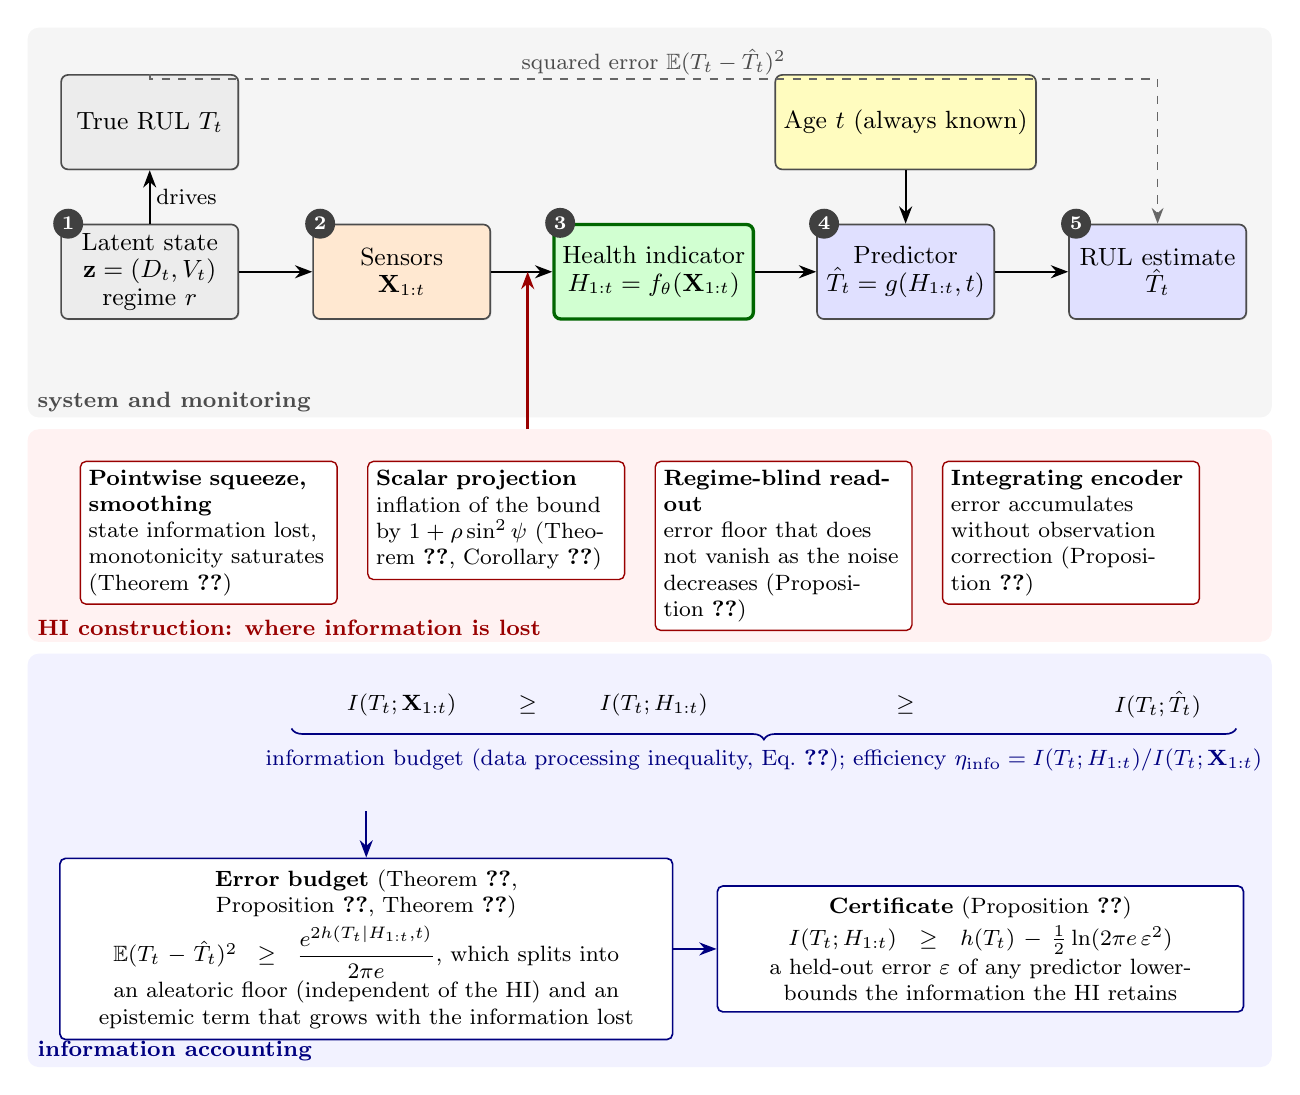
\begin{tikzpicture}[
  font=\small, >=Stealth,
  blk/.style={draw=black!70, rounded corners=2.5pt, minimum height=1.2cm, minimum width=2.25cm, align=center, fill=#1, line width=0.6pt, inner sep=3pt, drop shadow={shadow xshift=0.4pt,shadow yshift=-0.4pt,opacity=0.25}},
  lossbox/.style={draw=red!60!black, rounded corners=2pt, fill=white, align=left, font=\footnotesize, text width=3.05cm, inner sep=3pt, line width=0.5pt, minimum height=1.5cm, anchor=north},
  infobox/.style={draw=blue!50!black, rounded corners=2pt, fill=white, align=center, font=\footnotesize, inner sep=4pt, line width=0.6pt},
  arr/.style={-{Stealth[length=2.2mm]}, line width=0.8pt},
  lane/.style={rounded corners=4pt, draw=none, fill=#1},
  lanelab/.style={font=\footnotesize\bfseries, anchor=south west, inner sep=2pt},
  stage/.style={circle, fill=black!75, text=white, font=\scriptsize\bfseries, inner sep=1.2pt, minimum size=3.8mm},
  lab/.style={font=\footnotesize, inner sep=2pt}]
\begin{scope}[on background layer]
  \fill[lane=black!4]  (-0.35,-1.0) rectangle (15.45,3.95);
  \fill[lane=red!5]    (-0.35,-3.85) rectangle (15.45,-1.15);
  \fill[lane=blue!5]   (-0.35,-9.25) rectangle (15.45,-4.0);
\end{scope}
\node[lanelab,black!70] at (-0.3,-1.0) {system and monitoring};
\node[lanelab,red!60!black] at (-0.3,-3.85) {HI construction: where information is lost};
\node[lanelab,blue!50!black] at (-0.3,-9.25) {information accounting};
% ---------------- chain
\node[blk=gray!15] (z) at (1.2,0.85) {Latent state\\[-1pt]$\mathbf z=(D_t,V_t)$\\[-1pt]regime $r$};
\node[blk=orange!18] (x) at (4.4,0.85) {Sensors\\[-1pt]$\mathbf X_{1:t}$};
\node[blk=green!18!white,draw=green!40!black,line width=1.2pt] (h) at (7.6,0.85) {Health indicator\\[-1pt]$H_{1:t}=f_\theta(\mathbf X_{1:t})$};
\node[blk=blue!12] (g) at (10.8,0.85) {Predictor\\[-1pt]$\hat T_t=g(H_{1:t},t)$};
\node[blk=blue!12] (e) at (14.0,0.85) {RUL estimate\\[-1pt]$\hat T_t$};
\foreach \n/\i in {z/1,x/2,h/3,g/4,e/5} \node[stage] at ($(\n.north west)+(0.1,0.0)$) {\i};
\draw[arr] (z) -- (x); \draw[arr] (x) -- (h); \draw[arr] (h) -- (g); \draw[arr] (g) -- (e);
\node[blk=gray!15] (T) at (1.2,2.75) {True RUL $T_t$};
\node[blk=yellow!25,minimum width=2.6cm] (age) at (10.8,2.75) {Age $t$ (always known)};
\draw[arr] (z) -- node[lab,right]{drives} (T);
\draw[arr] (age) -- (g);
\draw[dashed,black!60,line width=0.6pt,-{Stealth[length=2mm]}] (T.north) -- (1.2,3.3) -- node[lab,above=-1pt,black!70]{squared error $\E(T_t-\hat T_t)^2$} (14.0,3.3) -- (e.north);
% ---------------- where information is lost
\node[lossbox] (l1) at (1.95,-1.55) {\textbf{Pointwise squeeze, smoothing}\\ state information lost, monotonicity saturates (Theorem~\ref{thm:paradox})};
\node[lossbox] (l2) at (5.6,-1.55) {\textbf{Scalar projection}\\ inflation of the bound by $1+\rho\sin^2\psi$ (Theorem~\ref{thm:angular}, Corollary~\ref{cor:rotation})};
\node[lossbox] (l3) at (9.25,-1.55) {\textbf{Regime-blind read-out}\\ error floor that does not vanish as the noise decreases (Proposition~\ref{prop:regime})};
\node[lossbox] (l4) at (12.9,-1.55) {\textbf{Integrating encoder}\\ error accumulates without observation correction (Proposition~\ref{prop:accum})};
\coordinate (m) at (6.0,0.85);
\draw[arr,red!60!black,line width=0.9pt] (6.0,-1.15) -- (6.0,0.85-0.0) ;
% ---------------- information budget
\node[lab] (ix) at (4.4,-4.65) {$I(T_t;\mathbf X_{1:t})$};
\node[lab] (ih) at (7.6,-4.65) {$I(T_t;H_{1:t})$};
\node[lab] (ie) at (14.0,-4.65) {$I(T_t;\hat T_t)$};
\node[lab] at (6.0,-4.65) {$\ge$}; \node[lab] at (10.8,-4.65) {$\ge$};
\draw[decorate,decoration={brace,amplitude=4pt,mirror},line width=0.6pt,blue!50!black] (3.0,-4.95) -- node[below=5pt,lab,blue!50!black]{information budget (data processing inequality, Eq.~\ref{eq:dpi}); efficiency $\etaPIE=I(T_t;H_{1:t})/I(T_t;\mathbf X_{1:t})$} (15.0,-4.95);
% ---------------- bounds
\node[infobox,text width=7.5cm] (b1) at (3.95,-7.75) {\textbf{Error budget} (Theorem~\ref{thm:bound}, Proposition~\ref{prop:age}, Theorem~\ref{thm:physics})\\[2pt] $\E(T_t-\hat T_t)^2\ \ge\ \dfrac{e^{2h(T_t\mid H_{1:t},t)}}{2\pi e}$, which splits into an aleatoric floor (independent of the HI) and an epistemic term that grows with the information lost};
\node[infobox,text width=6.4cm] (b2) at (11.75,-7.75) {\textbf{Certificate} (Proposition~\ref{cor:cert})\\[2pt] $I(T_t;H_{1:t})\ \ge\ h(T_t)-\tfrac12\ln(2\pi e\,\varepsilon^2)$\\[1pt] a held-out error $\varepsilon$ of any predictor lower-bounds the information the HI retains};
\draw[arr,blue!50!black] (b1.east) -- (b2.west);
\draw[arr,blue!50!black] (3.95,-6.0) -- (b1.north -| 3.95,0);
\end{tikzpicture}
}
\caption{Framework of the paper. The HI is constructed from the sensors, which are driven by the same latent state as the true RUL, and the predictor uses the HI and the age. The data processing inequality gives an information budget; the red boxes list the operations of HI construction whose information loss is quantified.}
\label{fig:framework}
\end{figure}

The paper answers these questions as follows.
\begin{enumerate}
\item \textbf{An information lower bound in nats} (Section~\ref{sec:limits}). The entropy-power bound on the RUL error turns the held-out error of any predictor into a lower bound on the information that the HI retains beyond the age (Theorem~\ref{thm:bound}). The bound is a transformation of the mean squared error: within one data set it ranks predictors exactly as the RMSE does, and the paper does not claim otherwise. It adds an absolute scale that is comparable across data sets ($0.1$~nat is an RMSE lower by about $10\%$), a negative control (a predictor that uses only the age cannot exceed zero, which shows whether the lifetime distribution behind the bound is valid) and, for Wiener degradation, a split of the error into an irreducible floor and a part that a better HI can remove (Section~\ref{sec:physbound}).
\item \textbf{Four ways in which an HI loses information} (Section~\ref{sec:losses}): template shrinkage, projection on a static scalar, regime-blind estimation, and integration without observation correction. Each is stated as a result with its engineering consequence.
\item \textbf{Tests on real data and a benchmark} (Sections~\ref{sec:realdata} and \ref{sec:empirical}) on turbofan engines and lithium-ion cells, including the number of run-to-failure units that the bound requires, and a comparison of learned encoders with simple indicators.
\item \textbf{Engineering guidance} (Section~\ref{sec:guidance}): a decision table and a four-step workflow.
\end{enumerate}
The ingredients are classical: the data processing inequality, the chain rules, the maximum-entropy property of the Gaussian and the entropy-power bound \cite{cover2006}; the inverse-Gaussian distribution \cite{chhikara1989}; Gaussian conditioning \cite{bishop2006}; the Kalman filter \cite{kalman1960,durbin2012}; and the variational bottleneck bound \cite{alemi2017}. What is new is their use, with the age-only control, to measure the HI-construction step, the four losses that this explains, and the number of run-to-failure units that the measurement requires.


\section{Information budget of a health indicator}
\label{sec:limits}
Let $T_t>0$ be the true RUL at inspection time (age) $t$, $\mathbf{X}_{1:t}\in\mathbb{R}^{d\times t}$ the accumulated history of $d$ sensors, and $H_{1:t}=f_\theta(\mathbf{X}_{1:t})$ the HI trajectory produced by a map $f_\theta$ with parameters $\theta$. Throughout, $h(\cdot)$ is differential entropy, $I(\cdot\,;\cdot)$ is mutual information (both in nats), $\E$ and $\Var$ are expectation and variance, and $\mathcal N(\mu,\sigma^2)$ is the normal distribution. Any RUL estimator $\hat T_t=g(H_{1:t})$ obeys the Markov chain $T_t \to \mathbf{X}_{1:t}\to H_{1:t}\to \hat T_t$, because the latent degradation state drives both $T_t$ and $\mathbf{X}_{1:t}$. The data processing inequality \cite[Sect.~2.8]{cover2006} gives
\begin{equation}
I(T_t;\mathbf{X}_{1:t}) \ge I(T_t;H_{1:t}) \ge I(T_t;\hat T_t),
\label{eq:dpi}
\end{equation}
with equality in the first inequality if and only if $H_{1:t}$ is a sufficient statistic of $\mathbf{X}_{1:t}$ for $T_t$ \cite[Sect.~2.9]{cover2006}.

\begin{theorem}[Information budget]
\label{thm:bound}
Assume that $h(T_t)$ and $I(T_t;\mathbf{X}_{1:t})$ are finite, and let $\hat T_t$ be an estimator with finite second moment and mean squared error (MSE) $\varepsilon^2=\E[(T_t-\hat T_t)^2]$. The information efficiency $\etaPIE$ below is defined when $I(T_t;\mathbf{X}_{1:t})>0$.\\
(a) \emph{Bound.} If $\hat T_t=g(H_{1:t})$, then
\begin{equation}
\varepsilon^2\;\ge\;\Binfo(H_{1:t}) := \frac{1}{2\pi e}\exp\!\big(2h(T_t\mid H_{1:t})\big)=\frac{1}{2\pi e}\exp\!\big(2h(T_t)-2I(T_t;H_{1:t})\big),
\end{equation}
$\Binfo(H_{1:t})\ge \mathcal{B}_{\min}:=\frac{1}{2\pi e}e^{2h(T_t\mid \mathbf{X}_{1:t})}$, and
\begin{equation}
\Binfo(H_{1:t})/\mathcal{B}_{\min}=\exp\!\big(2\,(1-\etaPIE(H_{1:t}))\,I(T_t;\mathbf{X}_{1:t})\big),\qquad \etaPIE(H_{1:t}):=\frac{I(T_t;H_{1:t})}{I(T_t;\mathbf{X}_{1:t})}\in[0,1].
\end{equation}
(b) \emph{Information lower bound.} Such an estimator satisfies
\begin{equation}
I(T_t;H_{1:t})\;\ge\;h(T_t)-\tfrac12\ln\!\big(2\pi e\,\varepsilon^2\big).
\end{equation}
(c) \emph{Age.} The age $t$ is always available to a predictor and is treated as a random variable over the inspection ages; $\E_t$ denotes the expectation over $t$ and $h(T_t\mid t)$ the entropy of the conditional distribution of $T_t$ given the age. If $\hat T_t=g(H_{1:t},t)$, then $\varepsilon^2\ge\frac1{2\pi e}\exp\!\big(2h(T_t\mid H_{1:t},t)\big)$, and the information that the HI adds to the age satisfies
\begin{equation}
I(T_t;H_{1:t},t)=I(T_t;t)+I(T_t;H_{1:t}\mid t),\qquad I(T_t;H_{1:t}\mid t)\ge\E_t\,h(T_t\mid t)-\tfrac12\ln\!\big(2\pi e\,\varepsilon^2\big).
\end{equation}
\end{theorem}
\begin{proof}[Proof sketch]
(a) Translation invariance of the entropy, the fact that conditioning does not increase entropy and the maximum-entropy property of the Gaussian give $\E[E^2]\ge e^{2h(T_t\mid H_{1:t})}/(2\pi e)$; the ratio follows from (\ref{eq:dpi}), and conditioning on $H_{1:t}=\mathsf h$ before averaging gives the sharper pointwise form. (b) rearranges (a). (c) applies (a) conditionally on $t$, averages, and uses Jensen's inequality for the concave logarithm. The full proof is in the Supplementary Material (Section~\ref{S-app:proofs}).
\end{proof}
Theorem~\ref{thm:bound} is the classical entropy-power bound on the error of an estimator \cite[Sect.~8.6]{cover2006}, used here to turn HI construction into an information budget; wherever the Bayesian Cram\'er--Rao bound applies, it is not weaker (Remark~\ref{S-rem:bcrb} in the Supplementary Material).

\paragraph{Interpretation} Because $\Binfo=e^{2h(T_t)-2I}/(2\pi e)$, an HI that retains $I$ nats about the RUL cannot support an RMSE below $e^{-I}$ times the bound for an HI that retains none: every $0.1$~nat lowers the bound on the RMSE by about $10\%$. Part (b) turns the held-out MSE of any predictor into a number of nats, the \emph{information lower bound}, which needs only the one-dimensional entropy $h(T_t)$, ranks HIs in the same order as the MSE and is negative, hence uninformative, when the predictor is inaccurate. Part (c) gives the relevant baseline. Since the age is always known, the reference for an HI is the RUL given the age, not the marginal RUL. A sensor-free predictor that uses only the age is a necessary baseline and a negative control, because it cannot attain a positive lower bound on the information beyond the age (Section~\ref{sec:cert}). If the predictor uses the age, bound (b) already contains the age, and the difference between the bounds of an HI-and-age predictor and of an age-only predictor is a difference of two lower bounds that bounds nothing about the information the HI adds; only (c) does. The efficiency $\etaPIE$ could in principle be estimated before any predictor is trained, but mutual-information estimates are unreliable on small data sets \cite{paninski2003} (Supplementary Material, Section~\ref{S-app:p1}).

\section{A physics-constrained error budget}
\label{sec:physbound}
Assume that after inspection the latent degradation follows $dD_s=\mu\,ds+\sigma_B\,dW_s$, where $W_s$ is a standard Wiener process, $\sigma_B>0$ the diffusion coefficient and $\mu>0$ a unit-specific drift (the random-effect formulation of \cite{gebraeel2005,wang2010}) and with absorbing threshold $D_{\rm fail}$. The prognostically relevant latent state is $\mathbf z=(D_t,\mu)$, where the inspection level $D_t$ is \emph{not} observed directly but only through $\mathbf{X}_{1:t}$. With $a=D_{\rm fail}-D_t>0$, the RUL is conditionally inverse-Gaussian \cite{folks1978,tweedie1957}, $T_t\mid\mathbf z\sim\mathcal{IG}(m(\mathbf z),\,a^2/\sigma_B^2)$ with mean $m(\mathbf z)=a/\mu$ and variance $a\sigma_B^2/\mu^3$ \cite{chhikara1989}, and $T_t$ is independent of $\mathbf{X}_{1:t}$ (hence of $H_{1:t}$) given $\mathbf z$. Here $\mathcal{IG}(\text{mean},\text{shape})$ denotes the inverse Gaussian distribution. Define the information efficiency about the mean RUL $m=m(\mathbf z)$ as $\eta_m(H):=I(m;H_{1:t})/I(m;\mathbf{X}_{1:t})\in[0,1]$.

\begin{theorem}[Physics-constrained bound]
\label{thm:physics}
Assume $h(m\mid\mathbf{X}_{1:t})$ and $I(m;\mathbf{X}_{1:t})$ are finite. For any estimator $\hat T_t=g(H_{1:t})$ with finite second moment,
\begin{equation}
\E[(T_t-\hat T_t)^2]\;\ge\;\underbrace{\E\!\left[\frac{a\,\sigma_B^2}{\mu^3}\right]}_{\mathcal{E}_{\rm aleatoric}}+\underbrace{\E_{H}\!\left[\frac{e^{2h(m\mid H_{1:t}=\mathsf{h})}}{2\pi e}\right]}_{\mathcal{E}_{\rm epistemic}},
\end{equation}
and the epistemic term obeys
\begin{equation}
\mathcal{E}_{\rm epistemic}\;\ge\;\frac{1}{2\pi e}\exp\!\Big(2h(m\mid\mathbf{X}_{1:t})+2\big(1-\eta_m(H)\big)\,I(m;\mathbf{X}_{1:t})\Big).
\end{equation}
The aleatoric term does not depend on the HI.
\end{theorem}
\begin{proof}[Proof sketch]
The cross term vanishes, so the squared error splits into $\E[\Var(T_t\mid\mathbf z)]$ and $\E[(m(\mathbf z)-\hat T_t)^2]$; Theorem~\ref{thm:bound} applied to $m(\mathbf z)$ conditionally on $H_{1:t}$ gives the epistemic term, and Jensen's inequality with $h(m\mid H)=h(m\mid\mathbf X)+(1-\eta_m)I(m;\mathbf X)$ gives the second bound of the theorem. The full proof is in the Supplementary Material (Section~\ref{S-app:proofs}).
\end{proof}
\begin{remark}
If the level $D_t$ were known, $a$ would be known and a change of variables would give $h(m\mid H,D_t)=h(\mu\mid H,D_t)+\E\ln(a/\mu^2)$. If the degradation followed the same constant-drift model from time $0$ with $D_0=0$ and $D_t$ were observed, $D_t/t$ would be a sufficient statistic for $\mu$ and the resulting bound would not depend on the HI. The HI matters through the joint uncertainty about the level and the drift, which is why Theorem~\ref{thm:physics} is stated for the latent pair $\mathbf z$. The second inequality of the theorem (the Jensen form) is weaker than the first but depends on the HI only through $\eta_m$.
\end{remark}

The bound of Theorem~\ref{thm:physics} is conservative by an exact non-Gaussianity gap, the expected posterior variance of the mean RUL multiplied by $1-e^{-2D}$, where $D$ is the Kullback--Leibler (KL) divergence of the posterior from a Gaussian with the same mean and variance (Proposition~\ref{S-prop:gap} in the Supplementary Material).

\paragraph{Numerical verification}
\label{sec:physnum}
The drift is $\mu\sim\mathcal N(1,0.22^2)$, truncated to $\mu>0.3$ and $a>1$, with $\sigma_B=0.85$, $D_{\rm fail}=100$ and $t=50$. The raw sensor is $X_k=D_k+\xi_k$ with $\xi_k\sim\mathcal N(0,1.5^2)$, and HIs with decreasing information are $H^{\varsigma}_k=X_k+\varsigma\zeta_k$ with standard normal $\zeta_k$ and $\varsigma\in\{0,2,4,8,16,32\}$. The posterior of $(D_t,\mu)$ is Gaussian (Kalman filter), $m=a/\mu$ is evaluated on $1500$ posterior draws for each of $1500$ test units, and the entropies are estimated with the Vasicek estimator \cite{vasicek1976}; the Bayes-optimal error is $\E[\Var(T_t\mid\mathbf z)]+\E[\Var(m\mid H)]$.

The aleatoric term is constant ($\approx63.8$ cycles$^2$), whereas the epistemic term grows as $\eta_m$ falls from $1$ to $0.38$ (Supplementary Table~\ref{S-tab:exp2}). The pointwise bound stays below the Bayes-optimal error at every noise level (RMSE $11.8$ against $12.3$ cycles for $\varsigma=0$, and $18.1$ against $19.6$ for $\varsigma=32$). The exact epistemic variance exceeds the pointwise value because the posterior of $m$ is not Gaussian (mean KL divergence $0.07$ nats at $\varsigma=0$, Proposition~\ref{S-prop:gap}). The marginal density of the Supplementary Material (Section~\ref{S-sec:pgib}) agrees with numerical integration to within $0.31\%$. Three independent repetitions with $1500$ units gave $59.7$ to $64.4$ cycles$^2$ for the aleatoric and $78.9$ to $87.2$ cycles$^2$ for the exact epistemic term at $\varsigma=0$, because $a/\mu$ has a heavy right tail, while the irreducible share stayed at $42$ to $43\%$; gaps of a few per cent between the columns of Supplementary Table~\ref{S-tab:exp2} should not be over-interpreted.

\paragraph{Engineering consequence} The aleatoric term is a floor that no HI can lower. In the example it is $64$ cycles$^2$ against $87$ cycles$^2$ of epistemic error for a lossless HI, so that about $42\%$ of the squared error is irreducible; comparing the achieved error of a predictor with this floor shows how much a better HI could still gain, and the epistemic term grows to $319$ cycles$^2$ when the HI retains only $38\%$ of the information in the sensors.

\section{Four ways in which an HI loses information}
\label{sec:losses}
An HI can lose information about the RUL in four ways that are common in practice: by template shrinkage that raises a geometric score (Section~\ref{sec:paradox}), by projection of the latent state on a static scalar (Section~\ref{sec:angular}), by ignoring the operating regime (Section~\ref{sec:regimeleak}) and by integrating an estimated velocity without correction from the observations (Section~\ref{sec:accum}). Each is stated as a result and checked on an exactly solvable model.

\subsection{Template shrinkage: geometric criteria do not measure information}
\label{sec:paradox}
The geometric criteria of Coble and Hines \cite{coble2009} are computed from the shape of the HI. Monotonicity is $\Mon(H_{1:t})=|\sum_{k=1}^{t-1}\mathrm{sgn}(H_{k+1}-H_k)|/(t-1)$, the balance of positive and negative increments. Prognosability is $\mathrm{Pro}=\exp(-\mathrm{std}(H_{\rm end})/\mathrm{mean}|H_{\rm end}-H_{\rm start}|)$, where the standard deviation and the mean are taken over units, $H_{\rm start}$ and $H_{\rm end}$ being the first and last values of each unit. In the benchmarks, $\mathrm{Tre}$ is the absolute correlation of the HI with time, as in \cite{javed2013} (and, under the name correlation, in \cite{zhang2016}); it differs from the trendability of Coble and Hines, which measures the agreement of the functional form across units \cite{coble2009}.

A strictly monotone bijection $\varrho$ satisfies $I(T_t;\varrho(H_{1:t}))=I(T_t;H_{1:t})$, so information can be lost only through non-injective operations or noise. We therefore consider $\tilde H_{1:t}=\mathcal S(H_{1:t},\xi)$, where $\xi$ is independent of everything else. We call $\mathcal S$ a \emph{template shrinkage} when it contracts the HI towards a template trajectory.

\begin{theorem}[Template shrinkage]
\label{thm:paradox}
(a) For any such $\mathcal S$, $T_t\to H_{1:t}\to\tilde H_{1:t}$ is Markov, so $I(T_t;\tilde H_{1:t})\le I(T_t;H_{1:t})$ and
\begin{equation}
\Binfo(\tilde H_{1:t})/\Binfo(H_{1:t})=\exp\!\big(2[I(T_t;H_{1:t})-I(T_t;\tilde H_{1:t})]\big)\ge 1 .
\end{equation}
(b) Let the HI be the level $D_k$ of a linear-Gaussian latent state, observed with Gaussian noise, $H_k=D_k+\xi^{(1)}_k$, and let the shrinkage with strength $\gamma\in[0,1)$ and template (mean trajectory) $m_k=\E[D_k]$ be
\begin{equation}
\begin{gathered}\tilde H_k^{\gamma}=m_k+(1-\gamma)(H_k-m_k)+\xi^{(2)}_k,\\ \xi^{(2)}_k\sim\mathcal N(0,\sigma_2^2)\ \text{independent and identically distributed (i.i.d.)}\end{gathered}
\end{equation}
For every linear functional $\vartheta$ of the latent state, for example the current velocity $V_t$, $\mathcal I^\vartheta_{\rm tot}(\gamma):=I(\vartheta;\tilde H^\gamma_{1:t})$ is non-increasing in $\gamma$ and
\begin{equation}
\mathcal I^\vartheta_{\rm tot}(\gamma)\xrightarrow[\gamma\to1]{}0.
\end{equation}
If the template has constant increment $\Delta m$, then, letting $\gamma\to 1$ and afterwards $t\to\infty$,
\begin{equation}
\Mon(\tilde H^{\gamma}_{1:t})\to \Mon_\infty=2\Phi_{\mathcal N}\!\big(\Delta m/(\sqrt2\,\sigma_2)\big)-1,
\end{equation}
where $\Phi_{\mathcal N}$ is the standard normal distribution function; the limit does not depend on the unit's own degradation.
\end{theorem}
\begin{proof}[Proof sketch]
Part (a) follows from the data processing inequality. In (b) the shrunk HI is an invertible affine image of $H$ observed through Gaussian noise whose variance grows without bound as $\gamma\to1$, so the information vanishes, and the limit of $\Mon$ follows from the strong law of large numbers for the 1-dependent increments. The full proof is in the Supplementary Material (Section~\ref{S-app:proofs}).
\end{proof}
Part (b) shows that the geometric score and the information content are decoupled. Once the shrinkage is strong, $\Mon$ saturates at a value set by the template and the noise, while the information available for RUL prediction keeps falling and the bound $\Binfo$ keeps rising. The loss splits into a part about the current state and a part about the kinematics (Proposition~\ref{S-prop:pointwise} in the Supplementary Material).

\paragraph{Numerical verification}
\label{sec:paradoxnum}
The latent state is a local linear trend, $D_k=D_{k-1}+V_{k-1}+\sigma_Bw_k$ and $V_k=V_{k-1}+\sigma_V\zeta_k$, with level $D_k$, velocity $V_k$ and standard normal noises $w_k,\zeta_k$. The raw HI is $H_k=D_k+\xi^{(1)}_k$ and the shrinkage is that of Theorem~\ref{thm:paradox}(b); the parameters, $400$ test units and three seeds are given in the Supplementary Material (Section~\ref{S-app:sim}). The information about $V_t$ is exact from the Kalman covariances \cite{kalman1960,durbin2012}, and $\sqrt{\Binfo}$ is the square root of the average of the pointwise entropy powers. Errors are reported as RMSE.

\begin{figure}[!tb]
\centering
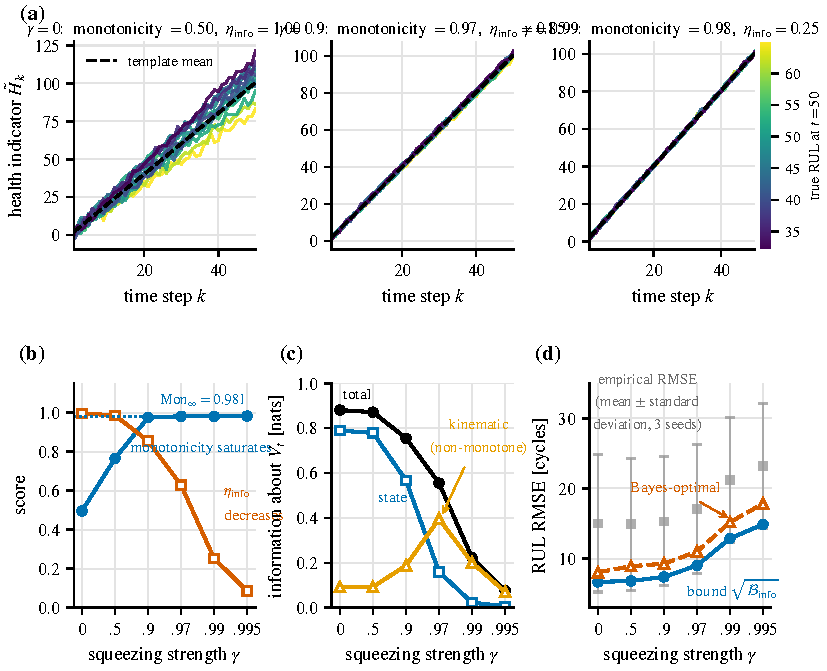
\includegraphics[width=\textwidth]{figs/fig_paradox}
\caption{Template-shrinkage experiment. (a) HI paths of 14 units, coloured by the true RUL. (b) Monotonicity and efficiency. (c) Information about $V_t$. (d) Bound and RMSE (error bars: standard deviation over seeds). The values of $\gamma$ are equally spaced.}
\label{fig:paradox}
\end{figure}

Monotonicity rises from $0.50$ to $0.98$ and saturates at the predicted value $\Mon_\infty=0.981$ for $\gamma\ge0.97$ (Supplementary Table~\ref{S-tab:exp1}, Figure~\ref{fig:paradox}), while from $\gamma=0.9$ to $0.995$ the efficiency (the information about $V_t$ that the shrunk HI retains relative to the HI before shrinkage) falls from $0.85$ to $0.09$ and the Bayes-optimal RMSE nearly doubles ($9.3$ to $17.8$ cycles). The bound stays below the Bayes-optimal error in every run. The state information falls monotonically, whereas the kinematic information first rises and then falls, so the increase of the bound at $\gamma=0.9$ and $0.97$ is driven by the loss of state information. The empirical RMSE varies strongly between seeds because of the heavy right tail of the RUL, and the posterior-based Bayes RMSE is the reliable summary.

\paragraph{Engineering consequence} Monotonicity, trendability and prognosability are not measures of information: an HI can be made to score higher by shrinking it toward a template while it loses information. They are not misleading by default: among candidate HIs derived from the sensors their ranking agreed with the information lower bound on turbofan engines but not reliably on lithium-ion cells (Section~\ref{sec:realdata}). Use them as screening scores and confirm the chosen HI by its information lower bound.

\subsection{Projection: scalar indicators at the trajectory level}
\label{sec:angular}
Theorem~\ref{thm:bound} concerns the information budget of an arbitrary HI. We now ask what a \emph{scalar}, \emph{static} HI loses when the degradation velocity varies in time. The loss has the same $\sin^2$ structure as the projection-misalignment loss at the snapshot level in \cite{le2026jestch}, but it acts along the \emph{temporal} direction (level versus velocity).

\paragraph{Setting} Let $\mathbf z=(D_t,V_t)^\top$ be the level and the velocity at inspection time $t$, with Gaussian prior $\mathcal N(\mathbf z_0,\boldsymbol\Sigma)$, observed through $\mathbf{X}_{1:t}$ in a linear-Gaussian model (for example the local-linear-trend state space \cite{harvey1989,durbin2012} of Section~\ref{sec:paradoxnum} with Gaussian sensor noise). The posterior is $\mathcal N(\hat{\mathbf z},\mathbf P)$ where $\hat{\mathbf z}=\E[\mathbf z\mid\mathbf{X}_{1:t}]$ and $\mathbf P$ does not depend on the data (as for the covariance recursion of the Kalman filter \cite{kalman1960,durbin2012}); $\hat{\mathbf z}\sim\mathcal N(\mathbf z_0,\boldsymbol\Lambda)$ with $\boldsymbol\Lambda=\boldsymbol\Sigma-\mathbf P\succ0$ (law of total variance \cite[Sect.~1.5.5]{bishop2006}), and $\hat{\mathbf z}$ is a sufficient statistic of $\mathbf{X}_{1:t}$ for $\mathbf z$. The target is the frozen-velocity RUL $m(\mathbf z)=(D_{\rm fail}-D_t)/V_t$, which is nonlinear in $\mathbf z$. We linearise it at a \emph{fixed}, non-random operating point $\bar{\mathbf z}=(\bar D,\bar V)^\top$, for example the prior mean at the inspection stage. Then
\begin{equation}
\mathbf g=\nabla m(\bar{\mathbf z})=-\frac{1}{\bar V}\Big(1,\ \frac{\bar a}{\bar V}\Big)^{\!\top},\qquad \bar a=D_{\rm fail}-\bar D,
\end{equation}
is a fixed vector, and $m_L(\mathbf z)=m(\bar{\mathbf z})+\mathbf g^\top(\mathbf z-\bar{\mathbf z})$ is a fixed linear functional of $\mathbf z$. All statements of this section are exact for $m_L$; the error of replacing $m$ by $m_L$ is not covered by the theorems and is examined numerically below. A scalar \emph{linear} HI built from the sufficient statistic, with fixed weights $\mathbf u$, is $h_{\mathbf u}=\mathbf u^\top\hat{\mathbf z}$. Define the signal-to-noise ratio $\rho=\mathbf g^\top\boldsymbol\Lambda\mathbf g/\mathbf g^\top\mathbf P\mathbf g$ and the $\boldsymbol\Lambda$-angle $\psi\in[0,\pi/2]$ between $\mathbf g$ and $\mathbf u$,
\begin{equation}
\cos\psi=\frac{|\mathbf g^\top\boldsymbol\Lambda\mathbf u|}{\sqrt{(\mathbf g^\top\boldsymbol\Lambda\mathbf g)(\mathbf u^\top\boldsymbol\Lambda\mathbf u)}}.
\end{equation}


\begin{theorem}[Angular loss relation]
\label{thm:angular}
In the setting above, for every fixed $\mathbf u\ne0$:\\
(a) $\Var(m_L\mid h_{\mathbf u})=\mathbf g^\top\mathbf P\mathbf g+(\mathbf g^\top\boldsymbol\Lambda\mathbf g)\sin^2\psi$.\\
(b) For the linearised target, with $\Binfo$, $\mathcal B_{\min}$ and $\eta_m$ defined as in Theorem~\ref{thm:bound} and Section~\ref{sec:physbound} with $m_L$ in place of $T_t$ and $m$, and with $I(m_L;\mathbf{X}_{1:t})=\tfrac12\ln(1+\rho)$,
\begin{equation}
\frac{\Binfo(h_{\mathbf u})}{\mathcal B_{\min}}=1+\rho\sin^2\psi,\qquad \eta_m(h_{\mathbf u})=1-\frac{\ln(1+\rho\sin^2\psi)}{\ln(1+\rho)} .
\end{equation}
(c) $\eta_m(h_{\mathbf u})=1$ if and only if $\mathbf u\parallel\mathbf g$; the HI $h_{\mathbf g}=\mathbf g^\top\hat{\mathbf z}$ is information-lossless for $m_L$ and is, by Lemma~\ref{S-lem:reduce} (Supplementary Material), the best scalar linear HI of $\mathbf{X}_{1:t}$.
\end{theorem}
\begin{proof}[Proof sketch]
Gaussian conditioning of $\mathbf g^\top\mathbf z$ on $h_{\mathbf u}$ gives (a); in the linearised model the entropy power equals the variance, and the mutual information of jointly Gaussian variables gives (b); (c) holds because $\sin\psi=0$ if and only if $\mathbf u\parallel\mathbf g$ ($\boldsymbol\Lambda\succ0$), and Lemma~\ref{S-lem:reduce} shows that no scalar linear functional of $\mathbf X$ does better. The full proof is in the Supplementary Material (Section~\ref{S-app:proofs}).
\end{proof}

\begin{remark}[Scope of the angular relation]
\label{rem:scope}
The theorem concerns scalar \emph{linear} HIs with fixed weights and the linearised target. If the operating point is replaced by the posterior mean $\hat{\mathbf z}$ of each unit, the gradient becomes a function of the data, and the theorem then describes the loss conditionally on freezing the gradient, that is, a local analysis around the unit's own estimate. An HI with unit-specific weights is a nonlinear scalar function of $\hat{\mathbf z}$ and is not covered by the optimality statements, which also do not exclude nonlinear scalar HIs with fixed structure.
\end{remark}

\begin{corollary}[No static scalar linear HI is optimal over the whole life]
\label{cor:rotation}
(a) In the coordinates $(D_t,V_t)$ the optimal direction is $\mathbf g_t\propto(1,\bar\tau_t)^\top$, with $\bar\tau_t=\bar a_t/\bar V_t$ the frozen-velocity RUL (in steps) at the operating point of stage $t$. The optimal scalar linear HI therefore weights the velocity estimate $\bar\tau_t$ times more than the level estimate; the weight moves from the velocity (early life, $\bar\tau_t$ large) to the level (end of life, $\bar\tau_t\to0$), and the Euclidean angle between the optimal directions at remaining lives $\tau_1,\tau_2$ is $|\arctan\tau_1-\arctan\tau_2|$.\\
(b) Let $\mathbf g_1,\mathbf g_2$ be the gradients at the operating points of two inspection stages with information matrices $\boldsymbol\Lambda_1,\boldsymbol\Lambda_2$ and ratios $\rho_1,\rho_2>0$. If $\mathbf g_1\not\parallel\mathbf g_2$, then for every fixed $\mathbf u$ the bound is increased at one of the two stages, $\max_j\rho_j\sin^2\psi_j(\mathbf u)\ge\delta>0$; if $\boldsymbol\Lambda_1=\boldsymbol\Lambda_2$, then $\delta\ge\min_j\rho_j\,\sin^2(\psi_{12}/2)$ with $\psi_{12}$ the $\boldsymbol\Lambda$-angle between $\mathbf g_1$ and $\mathbf g_2$. A stage-wise HI that uses the weights $\mathbf g_j$ at stage $j$ does not increase the bound, relative to the linearised target, at any stage.
\end{corollary}
\begin{proof}[Proof sketch]
Part (a) is the gradient formula above, and (b) follows from Theorem~\ref{thm:angular}(c), which makes the increase of the bound at stage $j$ vanish only for $\mathbf u\parallel\mathbf g_j$, and from the triangle inequality for the $\boldsymbol\Lambda$-angle between lines. The full proof is in the Supplementary Material (Section~\ref{S-app:proofs}).
\end{proof}
Corollary~\ref{cor:rotation}(a) explains why an indicator built from a level-like feature, for example the first principal component of cumulative-damage features, loses information early in life, and why a velocity-like feature loses it late in life. It is the temporal counterpart of the snapshot-level rotation of the signal direction. It also motivates the predictor of the Supplementary Material (Section~\ref{S-sec:fusion}), which uses both the smoothed HI level and its windowed slope: this pair estimates the two-dimensional sufficient statistic $\hat{\mathbf z}$.


\paragraph{Numerical verification}
\label{sec:angnum}
The model is the local linear trend of Section~\ref{sec:paradoxnum} with the raw sensor. For each of $500$ units, the exact entropy power of the \emph{nonlinear} target $m=(D_{\rm fail}-D_t)/V_t$ given $h_{\mathbf u}$ is estimated from the exact conditional Gaussian of $\mathbf z$ and compared with $1+\rho\sin^2\psi$ computed at a fixed operating point (the prior mean of the stage), as in Theorem~\ref{thm:angular}, and at the unit's own posterior mean (Remark~\ref{rem:scope}). As a consistency check, in the constant-drift model of Section~\ref{sec:physnum} the predicted factor is $1.000$ for every $\mathbf u$ (Monte Carlo $1.000$ to $1.003$), as the remark after Theorem~\ref{thm:physics} implies.

At $t=50$ both predictions agree with the Monte Carlo value within about $3\%$ for all HIs (Supplementary Table~\ref{S-tab:exp3}). The static HI aligned at $t^\ast=50$ is lossless at $t=25$ and $50$ but raises the bound by about $40\%$ at $t=75$ (Monte Carlo $1.39$), the level-only HI by about $37\%$ and the velocity-only HI by a factor of about $5$, which illustrates Corollary~\ref{cor:rotation}. The prediction at the fixed operating point underestimates the late-life increase for the static and the velocity-only HI ($1.12$ and $3.5$ at $t=75$), because the gradient of the nonlinear target at the prior mean differs from that at the units' own estimates; with the unit's own gradient ($1.40$ and $5.1$) the agreement is within $3\%$. The linear theory is thus an accurate local approximation, not an exact statement for the nonlinear target.

\paragraph{Engineering consequence} A static scalar HI is adequate only when the stage-optimal directions are close. Otherwise pass the level and the velocity of the HI to the predictor, as the windowed slope does in our predictor, or let the weights follow the stage of life.

\subsection{Regime-blind estimation}
\label{sec:regimeleak}
When the sensors are recorded under several operating regimes, the sensor responds to the degradation with a regime-dependent offset and gain, whereas the degradation process itself is the same. The following statement quantifies what a regime-blind estimator loses.

\begin{proposition}[Error floor of a regime-blind estimator]
\label{prop:regime}
Let a latent level $D$ with mean $\bar d$ and variance $v$ be observed through a sensor as $x=c_rD+o_r+\varepsilon$, where the regime $r$ takes $R$ values with probabilities $p_r$ independently of $D$ and of the noise $\varepsilon$ (variance $\sigma^2$); $c_r$ and $o_r$ are the gain and offset of regime $r$ (all $c_r\ne0$). Put $\bar c=\E c_r$ and $V_x:=\Var(x)=\E[c_r^2]\E[D^2]-(\bar c\bar d)^2+\Var(o_r)+2\bar d\,\mathrm{Cov}(c_r,o_r)+\sigma^2$. The best regime-blind linear estimator of $D$ from $x$ has mean squared error
\begin{equation}
\mathrm{MSE}_{\rm blind}=v-\frac{\bar c^2v^2}{V_x},\qquad\text{and}\qquad \mathrm{MSE}_{\rm blind}\xrightarrow[\sigma\to0]{}\ \frac{v\,[\Var(c_r)\,v+\Var(\bar d c_r+o_r)]}{\bar c^2v+\Var(c_r)\,v+\Var(\bar d c_r+o_r)}\ >0
\end{equation}
unless the regimes agree in $c_r$ and in $\bar d c_r+o_r$, whereas the estimator $(x-o_r)/c_r$ that knows the regime attains $\mathrm{MSE}_{\rm aware}=\sigma^2\sum_rp_r/c_r^2\to0$.
\end{proposition}
\begin{proof}[Proof sketch]
With $D$ independent of $r$, $\mathrm{Cov}(D,x)=\bar c\,v$ and $\Var(x)=V_x$, and the best linear estimator has error $v-\mathrm{Cov}(D,x)^2/\Var(x)$; the limit follows by expanding the moments at $\sigma=0$; given the regime, $(x-o_r)/c_r$ is unbiased with variance $\sigma^2/c_r^2$. The full proof is in the Supplementary Material (Section~\ref{S-app:proofs}).
\end{proof}
Normalising the sensors within each regime removes the regime offsets but not the regime-dependent gains, so the floor remains. In a numerical example with six regimes ($c_r\in[0.6,1.6]$, $o_r\in[-0.5,0.6]$, $v=0.08$), the formula and a simulation agree on $\mathrm{MSE}_{\rm blind}=0.060$ at $\sigma=0$, so that only $25\%$ of $\Var(D)$ is explained, whereas the regime-aware estimator has an error that tends to zero.
\paragraph{Engineering consequence} Normalise the sensors by operating regime and, when protocols differ between units, by each unit's own early cycles. Per-regime normalisation removes offsets but not gains, so the regime should also be given to the observation model when gains differ.

\subsection{Integration without observation correction}
\label{sec:accum}
An HI that integrates an estimated velocity $u_k$, $H_k=H_{k-1}+u_k$, has nothing that anchors its level to the observations. Section~\ref{sec:angular} treats the level and the velocity as latent quantities, and the level must be re-estimated from the sensors at every step; this is the measurement update of a Kalman filter \cite{kalman1960}. An observation-corrected HI adds a direct level estimate $l_k$ and a gain $\omega_k\in(0,1)$, $H_k=(1-\omega_k)(H_{k-1}+u_k)+\omega_k\,l_k$, and $\omega=0$ is the pure integrator. The next proposition quantifies what the integrator accumulates.

\begin{proposition}[Error accumulation without observation correction]
\label{prop:accum}
Let the velocity estimate carry the error $e_k=b+w_k$ with a unit-specific persistent bias $b$ and white noise $w_k$ of variance $\sigma_w^2$, and let the direct level estimate $l_k$ carry independent zero-mean noise $n_k$ of variance $\sigma_n^2$. Let $\varepsilon_k$ be the error of the HI level. Conditionally on $b$, the pure integrator ($\omega=0$) has at step $t$ an error with mean $tb$ and variance $t\sigma_w^2$, both unbounded in $t$. For a constant gain $\omega\in(0,1]$ the error converges to a stationary distribution $\varepsilon_\infty$ with
\begin{equation}
\E\,\varepsilon_\infty=\frac{(1-\omega)\,b}{\omega},\qquad \Var\,\varepsilon_\infty=\frac{(1-\omega)^2\sigma_w^2+\omega^2\sigma_n^2}{\omega(2-\omega)} .
\end{equation}
\end{proposition}
\begin{proof}[Proof sketch]
The level error obeys $\varepsilon_k=(1-\omega)(\varepsilon_{k-1}+e_k)+\omega n_k$, so its mean and variance satisfy first-order recursions with the stated fixed points. The full proof is in the Supplementary Material (Section~\ref{S-app:proofs}).
\end{proof}
A simulation ($b=0.01$, $\sigma_w=0.02$, $\sigma_n=0.15$, $400$ steps, $2\times10^5$ paths) agrees with both expressions (for $\omega=0$ the bias is $4.00=tb$; for $\omega=0.2$ the bias and variance are $0.0399$ and $0.00321$ against $0.04$ and $0.00321$). A constant gain amounts to exponential smoothing, the steady state of the local-level filter \cite{harvey1989,durbin2012}. A persistent velocity bias is the generic situation when units differ in initial offset or wear, and it is consistent with the behaviour of the integrating encoder on the turbofan data, whose error falls once the correction is added (Section~\ref{sec:empirical}).
Two learned encoders implement this correction with a learned gain: PGIB-KF, an observation-corrected (Kalman-filter-based) variant of the physics-guided information bottleneck (PGIB), and its regime-aware variant PGIB-KFR. They are described in the Supplementary Material (Section~\ref{S-sec:pgib}) and compared with simple HIs in Section~\ref{sec:empirical}.

\paragraph{Engineering consequence} An encoder that integrates a velocity needs an observation correction: a gain on a direct level estimate turns an unbounded error into a bounded one.

\section{Tests on real data}
\label{sec:realdata}
This section tests the predictions of Sections~\ref{sec:limits} to \ref{sec:losses} directly, on two domains with many units: turbofan engines (the four subsets FD001 to FD004 of the Commercial Modular Aero-Propulsion System Simulation (C-MAPSS) data, 100 to 260 training engines) and lithium-ion cells (the HUST, MATR and Tongji collections, with 77, 169 and 88 cells). Estimators are compared in Section~\ref{sec:empirical}.

\subsection{Data and design}
All analyses use unit-grouped five-fold cross-validation: preprocessing, HIs and predictors are fitted on the training units of a fold and evaluated on its held-out units. The population consists of pairs of a unit and an age $t$ between a minimum age ($30$ cycles for engines, $100$, $50$ and $30$ cycles for the HUST, MATR and Tongji cells) and the age at which $10\%$ of the training units are still alive. Pooling all ages of all units gives $T_t\mid t$ the distribution of $L-t$ given $L>t$, where $L$ is the lifetime of a unit, so that $h(T_t\mid t)$ is estimated from the lifetime distribution of the training units (Gaussian kernel density of $\ln L$) without further assumption; $\bar h(T_t\mid t)$ denotes its average over the pairs, the quantity $\E_t\,h(T_t\mid t)$ of Theorem~\ref{thm:bound}(c). Predictors are gradient-boosted trees on summaries of the HI trajectory and the age, and confidence intervals are bootstrap intervals over units (Supplementary Material, Section~\ref{S-app:realdata}).

\paragraph{Turbofan engines} The training sets of the four C-MAPSS subsets are used (FD001 and FD003: one operating regime; FD002 and FD004: six regimes), with $14$ informative sensors standardised within regime where there are several. The HIs are a ridge regression of the life fraction (age divided by lifetime) on the standardised sensors (ridge HI) and the first principal component of the sensors (PCA-HI); a predictor on the raw sensors is the reference.

\paragraph{Lithium-ion cells} The HUST collection (Huazhong University of Science and Technology) \cite{ma2022} has 77 lithium iron phosphate/graphite cells, each cycled under its own protocol, with end of life at $80\%$ of the initial capacity ($977$ to $2334$ cycles). The MATR collection \cite{severson2019,attia2020} has 169 cells of the same chemistry under fast-charging protocols, with end of life at $80\%$ of the nominal capacity ($147$ to $2235$ cycles). The Tongji collection \cite{zhu2022} has 88 cells (of 130 recorded) of three nickel-based chemistries cycled at 25, 35 and 45~$^\circ$C, with end of life at $80\%$ of the nominal capacity ($121$ to $570$ cycles); the other cells did not reach this threshold or had lifetimes shorter than $100$ cycles. The collections were taken from the processed BatteryLife repository \cite{tan2025}. The HIs use only charging-phase features (charge duration and charge voltage at $27\%$ and $73\%$ of the nominal capacity), each relative to cycles 2 to 11 of the same cell; the discharge capacity, which defines the end of life, enters only a reference predictor (Supplementary Material, Section~\ref{S-app:realdata}).

\subsection{Age-conditional information lower bound}
\label{sec:cert}
\paragraph{Turbofan engines (Theorem~\ref{thm:bound}(c))} The information lower bound is $\bar h(T_t\mid t)-\tfrac12\ln(2\pi e\,\mathrm{MSE})\le I(T_t;H_{1:t}\mid t)$. A predictor that uses only the age is a negative control, since its lower bound cannot exceed zero when the lifetime distribution is correct; it is $-0.22$ to $-0.11$ nats on FD001 to FD004 (Table~\ref{tab:cmp}). The HI trajectory carries information beyond the age (Figure~\ref{fig:rda}(a)): the lower bound for the ridge HI is $0.10$ to $0.31$ nats, with $95\%$ intervals excluding zero except on FD003. Level-only and slope-only summaries of the same HI give lower bounds below that of the full trajectory on all four subsets. A predictor on the raw sensors gives $0.16$ to $0.25$ nats, similar to the supervised HI and higher on FD003 and FD004, so the HI is a compression of the sensors that retains at best the information they contain, not an addition to it. With $100$ or more engines the lower bound is positive and passes its control.

\paragraph{Lithium-ion cells} The age-only control is at or below zero on HUST and MATR and $0.05$ nats on Tongji, whose interval includes zero, and the lower bound for the ridge HI is $0.30$ to $0.60$ nats with intervals above zero (Figure~\ref{fig:rda}(a), Table~\ref{tab:cmp}). The three charging features used directly give higher lower bounds ($0.61$ to $0.91$ nats) than the scalar HI constructed from them, as the data processing inequality requires, and the capacity reference does not exceed them.

\paragraph{Small data sets} On the seven small battery and bearing sets of Section~\ref{sec:empirical} the model-based age-conditional bound fails the negative control on four of them, because a log-normal lifetime distribution fitted to three to seven lifetimes overestimates $h(T_t\mid t)$ (Supplementary Material, Table~\ref{S-tab:certage}). Among the data sets tested, the bound was positive and passed its control only with $77$ or more units; subsets of the larger sets put the threshold near $40$ (Section~\ref{sec:fleet}).

\subsection{Template shrinkage}
\paragraph{Turbofan engines (Theorem~\ref{thm:paradox})} Shrinkage toward the mean HI trajectory of the training engines, with noise chosen as in Section~\ref{sec:paradoxnum}, raises the monotonicity of the ridge HI from $0.13$--$0.24$ to $0.41$--$0.58$, where it saturates for $\gamma\ge0.97$ at the value predicted from the template ($0.41$--$0.58$ observed against $0.41$--$0.61$ predicted; Figure~\ref{fig:rda}(b)). Over the same range the information lower bound falls from $0.10$--$0.31$ nats to about zero or below (Figure~\ref{fig:rda}(c)).

\paragraph{Lithium-ion cells} Template shrinkage raises the monotonicity of the ridge HI from $0.32$ to $0.81$ on HUST, from $0.39$ to $0.48$ on MATR and from $0.65$ to $0.73$ on Tongji, close to the predicted limits ($0.82$, $0.49$ and $0.70$), while the lower bound falls to about zero or below on all three (Figure~\ref{fig:rda}(b,c)). In both domains, monotonicity and the information lower bound are decoupled.

\subsection{Geometric scores and information lower bound}
The template shrinkage above is a constructed example. To see whether geometric scores agree with the information bound among realistic HIs, each data set was given $42$ candidate HIs (40 random linear combinations of the normalised sensors or charging features, the PCA-HI and the ridge HI), and the score $\Mon+\mathrm{Tre}+\mathrm{Pro}$ was compared with the age-conditional information lower bound (Supplementary Material, Section~\ref{S-app:realdata}). On the four turbofan subsets the two agree: the Spearman correlation is $0.64$ to $0.97$, with bootstrap intervals above $0.4$, and the HI with the highest score ranks first or second of $42$ by its information lower bound (Table~\ref{tab:geom}). On the cells the results are inconsistent. On HUST and Tongji the correlation is indistinguishable from zero ($0.08$ and $0.16$), and on MATR it is $0.74$. On all three, however, the highest-score HI ranks only $18$th, $8$th and $16$th, with lower bounds of $0.28$, $0.25$ and $0.56$ nats against $0.57$, $0.43$ and $0.84$ for the best HI, that is, about half to two thirds. Geometric scores are therefore a reasonable screen on the engines and not reliable on the cells; we did not investigate the cause.

\begin{table}[!t]
\caption{Geometric score versus information lower bound over $42$ candidate HIs per data set. $\rho_{\rm S}$: Spearman correlation with the information lower bound ($95\%$ bootstrap interval over HIs).}
\label{tab:geom}
\centering\scriptsize
\adjustbox{max width=\linewidth}{\begin{tabular}{l c c c c c}
\hline
Data set & HIs & $\rho_{\rm S}$ (score) & $\rho_{\rm S}$ (Mon) & rank of the highest-score HI & certificate: highest-score HI / best HI \\
\hline
FD001 & 42 & 0.97 & 0.85 & 2 & 0.23 / 0.30 \\
FD002 & 42 & 0.89 & 0.59 & 1 & 0.21 / 0.21 \\
FD003 & 42 & 0.82 & 0.58 & 1 & 0.15 / 0.15 \\
FD004 & 42 & 0.64 & 0.59 & 1 & 0.20 / 0.20 \\
HUST & 42 & 0.08 & 0.52 & 18 & 0.28 / 0.57 \\
MATR & 42 & 0.74 & 0.75 & 8 & 0.25 / 0.43 \\
Tongji & 42 & 0.16 & 0.18 & 16 & 0.56 / 0.84 \\
\hline
\end{tabular}
}
\end{table}

\subsection{Direction of a scalar linear HI}
\paragraph{Turbofan engines (Theorem~\ref{thm:angular}, Corollary~\ref{cor:rotation})} For the level and the velocity of the ridge HI, the direction of the best linear scalar combination for the RUL, measured as the angle from the level axis, moves across stages (between $21^\circ$ and $56^\circ$ across age stages on FD002). Level-only and velocity-only HIs lose up to $20\%$ and $38\%$ of RMSE relative to the best direction chosen separately at each stage (Figure~\ref{fig:rdb}(b,c)), but the best \emph{static} direction, combined with a stage-specific affine map, loses at most $4\%$. The relation of Section~\ref{sec:angular} is consistent with the observed rotation, but its consequence is small on these data; the factor $1+\rho\sin^2\psi$ also depends on the signal-to-noise ratio $\rho$, which was not estimated here.

\paragraph{Lithium-ion cells} On HUST the optimal direction moves from $71^\circ$--$80^\circ$ in the first three life stages to $3^\circ$--$16^\circ$ in the last two, and the best static direction loses up to $9\%$ of RMSE in a stage ($18\%$ in the last age stage), against up to $54\%$ for velocity alone. On MATR a static direction loses at most $1.2\%$; on Tongji at most $3\%$ across life stages and $7\%$ across age stages. The loss predicted by the angular relation is thus material for HUST, modest for Tongji and negligible for MATR and for engines.

\subsection{Operating regime and test protocol}
\paragraph{Turbofan engines (Proposition~\ref{prop:regime})} For a linear estimator of the life fraction, regime blindness increases the RMSE from $0.137$ to $0.148$ on FD002 and from $0.165$ to $0.199$ on FD004 ($8\%$ and $21\%$); with one regime the three estimators coincide. Per-regime normalisation removes most of the loss, and regime-specific weights add only $1\%$, so the residual effect of heterogeneous gains is small in these data.

\paragraph{Lithium-ion cells} A linear estimator of the life fraction from the raw charging features, standardised over the population, has an RMSE of $0.136$ on HUST and $0.179$ on MATR; expressing each feature relative to the own early cycles of the cell, which removes the protocol- and cell-specific level, lowers it to $0.115$ and $0.142$ ($18\%$ and $26\%$), and from $0.190$ to $0.167$ ($14\%$) on Tongji. This is the analogue of regime normalisation of Proposition~\ref{prop:regime}, with the cell corresponding to the regime.

\subsection{What the information lower bound adds to the RMSE}
The RMSE in cycles cannot be compared across data sets (the age-only predictor has $45$ to $328$ cycles, Table~\ref{tab:cmp}). The gain in the information lower bound over the age-only predictor is exactly $\ln(\mathrm{RMSE}_{\rm age}/\mathrm{RMSE}_{\rm HI})$, so a gain of $0.3$ nats is an RMSE lower by about $26\%$ on every data set. Within one data set the bound ranks predictors exactly as the RMSE does and adds no new ranking. It adds two things. First, an absolute check: the age-only predictor cannot exceed zero if the lifetime distribution is correct. Its value shows how conservative the bound is ($-0.27$ nats on MATR, $-0.02$ on HUST), and it indicated the mismatch between the training distribution and the FD003 test engines ($+0.33$ nats), which no comparison of RMSE values would have revealed. Second, an information reading that applies to any predictor, including an end-to-end one (Section~\ref{sec:empirical}).

\begin{table}[!t]
\caption{RMSE and information lower bound of the age-only predictor and of the ridge HI (cross-validation). Gain: difference of the information lower bounds, equal to $\ln$ of the RMSE ratio.}
\label{tab:cmp}
\centering\scriptsize
\adjustbox{max width=\linewidth}{\begin{tabular}{l c c c c c c c}
\hline
Data set & Median life & \multicolumn{3}{c}{RMSE [cycles]} & \multicolumn{3}{c}{Certificate [nats]} \\
 & [cycles] & age only & ridge HI & ratio & age only & ridge HI & gain \\
\hline
FD001 & 199 & 45 & 29 & 0.66 & -0.11 & 0.31 & 0.42 \\
FD002 & 199 & 45 & 33 & 0.73 & -0.11 & 0.21 & 0.32 \\
FD003 & 220 & 85 & 62 & 0.73 & -0.22 & 0.10 & 0.32 \\
FD004 & 234 & 68 & 51 & 0.74 & -0.12 & 0.18 & 0.30 \\
HUST & 1708 & 301 & 218 & 0.72 & -0.02 & 0.30 & 0.32 \\
MATR & 760 & 328 & 181 & 0.55 & -0.27 & 0.32 & 0.60 \\
Tongji & 363 & 92 & 53 & 0.58 & 0.05 & 0.60 & 0.55 \\
\hline
\end{tabular}
}
\end{table}

\subsection{Number of units needed}
\label{sec:fleet}
Estimating the information lower bound requires run-to-failure units, so an engineer must know how many. Random subsets of $k$ units were drawn from each data set ($10$ subsets per size), the unit-grouped cross-validation was repeated on each, and a subset was called \emph{valid} when the ridge HI exceeded the age-only predictor by more than $0.1$ nat while the control stayed at or below $0.05$ nat (Table~\ref{tab:fleet}). With $5$ units the share of valid subsets was $0.2$ to $0.5$; with $40$ units it was $0.9$ to $1.0$, except $0.7$ on FD004 and $0.1$ on Tongji. Tongji did not reach a valid share in subsets of up to $40$ cells because its age-only control stayed at $0.11$ to $0.22$ nats and fell to $0.05$ only with all $88$ cells; its three chemistries and temperatures make the lifetime distribution harder to estimate. The number of units needed thus depends on the heterogeneity of the fleet, and the control must be checked in every case. The thresholds are conventions, so the result is an order of magnitude: about $40$ units for a decision, and fewer than $10$ units are unreliable.

\begin{table}[!t]
\caption{Share of valid random subsets of $k$ units (mean gain in the information lower bound over the age-only control, in nats, in brackets); $10$ subsets per size, `--' if $k$ exceeds $80\%$ of the units.}
\label{tab:fleet}
\centering\scriptsize
\adjustbox{max width=\linewidth}{\begin{tabular}{l c c c c c c }
\hline
Data set & $k=5$ & $k=10$ & $k=20$ & $k=40$ & $k=80$ & $k=120$ \\
\hline
FD001 & 0.5 (0.10) & 0.6 (0.17) & 0.7 (0.16) & 1.0 (0.26) & 1.0 (0.33) & -- \\
FD002 & 0.4 (0.08) & 0.5 (0.08) & 0.7 (0.14) & 1.0 (0.21) & 1.0 (0.22) & -- \\
FD003 & 0.4 (-0.05) & 0.4 (0.11) & 0.6 (0.19) & 1.0 (0.25) & 1.0 (0.34) & -- \\
FD004 & 0.3 (-0.06) & 0.4 (0.06) & 0.3 (0.08) & 0.7 (0.14) & 1.0 (0.24) & -- \\
HUST & 0.2 (-0.09) & 0.3 (0.12) & 0.6 (0.13) & 0.9 (0.26) & -- & -- \\
MATR & 0.3 (0.06) & 0.7 (0.32) & 1.0 (0.30) & 0.9 (0.42) & 1.0 (0.44) & 1.0 (0.57) \\
Tongji & 0.2 (0.30) & 0.0 (0.20) & 0.0 (0.19) & 0.1 (0.41) & -- & -- \\
\hline
\end{tabular}
}
\end{table}

\subsection{Sensitivity to the inclusion rule on Tongji}
Excluding the $33$ of the $130$ recorded Tongji cells that never reached the end-of-life threshold removes long-lived cells (right censoring); counting the $31$ of them with at least $100$ recorded cycles as failed at their last recorded cycle biases the lifetimes downward, so the two rules bound the effect (Supplementary Material, Table~\ref{S-tab:senstongji}). The age-only control still passes ($-0.04$ nats) and the ridge HI still carries information beyond the age (lower bound $0.31$ nats, interval $0.23$ to $0.43$), but the bound halves from $0.60$, the loss of a static direction rises from $7\%$ to $9\%$, and the protocol effect falls from $14\%$ to $5\%$. The qualitative conclusions hold; the size of the effects on Tongji depends on how censored cells are treated.

\begin{figure}[!tb]
\centering
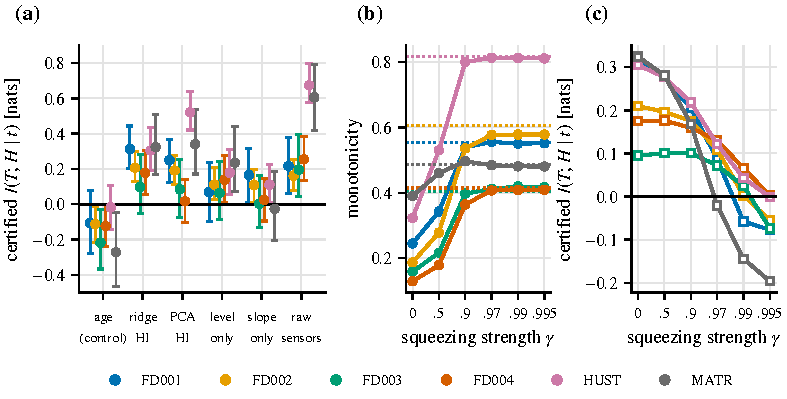
\includegraphics[width=\textwidth]{figs/fig_realdata_a}
\caption{Cross-validated tests on turbofan engines (FD001--FD004) and lithium-ion cells (HUST, MATR, Tongji). (a) Lower bound on $I(T_t;H_{1:t}\mid t)$ for HI summaries, with $95\%$ bootstrap intervals. (b) Monotonicity and (c) the information lower bound after template shrinkage of strength $\gamma$; dotted lines: predicted $\mathrm{Mon}_\infty$.}
\label{fig:rda}
\end{figure}

\begin{figure}[!tb]
\centering
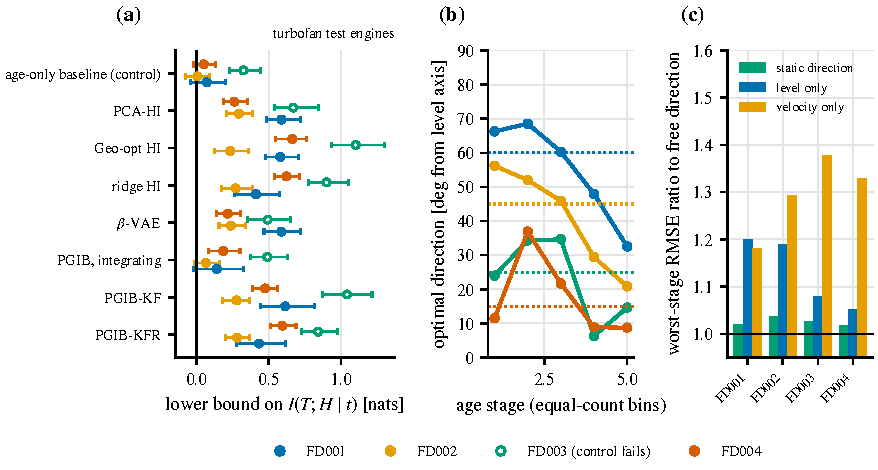
\includegraphics[width=\textwidth]{figs/fig_realdata_b}
\caption{(a) Information lower bounds of the benchmark methods on the official turbofan test engines (hollow markers: age-only control fails). (b) Optimal direction of a scalar linear HI per age stage; dotted: best static direction. (c) Worst-stage RMSE ratio to the direction chosen separately at each stage.}
\label{fig:rdb}
\end{figure}

\section{Benchmark of estimators}
\label{sec:empirical}
Section~\ref{sec:realdata} tests the theory with generic HIs. This section asks what the theory implies for estimators, and makes three predictions that run-to-failure data can test. (i) A sensor-free predictor that uses only the age should be competitive when the sensors are weak (Theorem~\ref{thm:bound}(c)). (ii) An integrating encoder accumulates error and an observation-corrected one does not (Proposition~\ref{prop:accum}). (iii) Learned encoders have a training variance that must be measured before differences between HIs are interpreted.

\paragraph{Design} Three simple HIs (the first principal component, PCA-HI; a combination optimised for the geometric criteria, Geo-opt HI; and a supervised ridge regression, ridge HI) are compared with three learned encoders (a $\beta$-variational autoencoder, $\beta$-VAE; a variational information bottleneck without physics prior, VIB; and the PGIB with its Kalman-corrected variant PGIB-KF and its regime-aware variant PGIB-KFR; Supplementary Material, Section~\ref{S-sec:pgib}). All HIs feed the \emph{same} calibrated predictor (Section~\ref{S-sec:fusion}); the \emph{age-only baseline} is that predictor without the HI, that is, the lifetime distribution of the training units conditioned on survival to the current age. The data are battery cells (NASA PCoE, CALCE CS2) and bearings (FEMTO-ST, IMS) with three to seven units each, evaluated leave-one-unit-out, and the four C-MAPSS subsets, evaluated on the official test engines. The Supplementary Material gives the data, the evidence tiers (independent confirmations and development results), the protocol history and the full tables (Section~\ref{S-app:data}).

\paragraph{Age-only baseline with few training units (prediction i)} With two to six training units no method is best everywhere: the age-only baseline has the lowest RMSE on both FEMTO conditions and is within a factor of $1.5$ of the best method on six of the seven sets (Supplementary Figure~\ref{S-fig:smalls}). On C-MAPSS the sensors are far more informative: the age-only baseline has an RMSE of $36.6$ to $54.7$ cycles, against $21.8$ to $29.7$ for the best simple HI. The age-only baseline is thus a competitive baseline where the sensors are weak, and it must be reported.

\paragraph{Error accumulation and its correction (prediction ii)} With $80$ to $208$ training engines, the integrating encoder performs considerably worse than the best simple HI (single-model RMSE $34.8$ to $48.7$ against $21.8$ to $29.7$) and only $2$ to $6$ RMSE units below the age-only baseline. The observation-corrected PGIB-KF reduces the RMSE to $23.8$--$40.7$ for a single model and to $21.3$--$35.8$ for a ten-seed ensemble (Supplementary Table~\ref{S-tab:var10}). The deficit is therefore not caused by the bottleneck objective, which is the same in both models, but by the missing anchoring of the level.

\paragraph{Information lower bounds of the benchmark methods} On the official test engines (Figure~\ref{fig:rdb}(a)) the lower bounds give an information-theoretic reading of the error accumulation of Proposition~\ref{prop:accum}. On FD001, FD002 and FD004 the age-only baseline passes the control ($0.07$, $0.01$ and $0.05$ nats). The integrating PGIB reaches only $0.14$, $0.07$ and $0.19$ nats, close to the baseline on FD001 and FD002, whereas PGIB-KF reaches $0.61$, $0.28$ and $0.48$ nats and the best simple HI $0.59$, $0.29$ and $0.66$ nats. On FD003 the control fails ($0.33$ nats): the lifetime distribution of the training engines does not describe the test population, and the FD003 values are not interpreted.

\paragraph{Maintenance decision at fixed risk} For each test engine the replacement is scheduled at the predicted RUL plus a margin, the residual quantile of the method that makes $5\%$ (or $10\%$) of the engines fail; the margin is cross-fitted over engines, and the unused life is the true RUL minus the scheduled time. The age-only baseline leaves $50$ to $77$ cycles unused (Table~\ref{tab:decision}). The best simple HI, chosen afterwards on each subset, reduces this by $45$, $23$, $43$ and $43\%$ on FD001 to FD004 (intervals above zero), whereas the integrating PGIB leaves $0$ to $12\%$ less than the baseline, with an interval that includes zero on FD001 to FD003. The evaluation is simplified (one decision per engine, no real maintenance costs), but it shows that the information quantified by the bound translates into usable life, and that the integrating encoder yields little of it.

\begin{table}[!t]
\caption{Unused life [cycles] at fixed failure risk on the official test engines (replacement scheduled at the predicted RUL plus a cross-fitted margin that makes $5\%$ or $10\%$ of the engines fail).}
\label{tab:decision}
\centering\scriptsize
\adjustbox{max width=\linewidth}{\begin{tabular}{l c c c c c c c c}
\hline
& \multicolumn{4}{c}{5\% of engines fail} & \multicolumn{4}{c}{10\% of engines fail} \\
Method & FD001 & FD002 & FD003 & FD004 & FD001 & FD002 & FD003 & FD004 \\
\hline
Age law & 50 & 54 & 59 & 77 & 44 & 46 & 49 & 67 \\
PCA-HI & 28 & 45 & 60 & 74 & 24 & 35 & 44 & 63 \\
Geo-opt HI & 27 & 42 & 33 & 44 & 24 & 32 & 24 & 34 \\
Ridge HI & 36 & 42 & 37 & 49 & 30 & 32 & 29 & 39 \\
PGIB, integrating & 49 & 53 & 59 & 68 & 42 & 45 & 51 & 62 \\
PGIB-KF & 34 & 46 & 33 & 56 & 25 & 33 & 28 & 45 \\
\hline
\end{tabular}
}
\end{table}

\paragraph{Comparison with an end-to-end predictor} A gradient-boosting predictor on all $14$ sensors reaches an RMSE of $24.7$, $26.4$, $31.6$ and $34.0$ with the true RUL as target and $13.6$, $25.1$, $13.5$ and $26.0$ with the target clipped at $125$ cycles, against $21.8$, $28.7$, $21.9$ and $29.7$ for the best scalar-HI predictor (Table~\ref{tab:e2e}). With the unclipped target the scalar HI is better except on FD002; with the clipped target the end-to-end predictor is $38\%$ better on the single-regime subsets and about $12\%$ better on the multi-regime ones. The information lower bound applies to the end-to-end predictor as well, and its excess over the best scalar HI ($0.47$, $0.14$, $0.49$ and $0.13$ nats; the FD003 values are overestimated because of the lifetime-distribution mismatch) is the information lost by compressing the sensors into one scalar. A scalar HI is therefore justified by interpretability and threshold-based failure models, not by accuracy alone.

\begin{table}[!t]
\caption{Scalar-HI predictors and an end-to-end predictor on all sensors, official C-MAPSS test engines.}
\label{tab:e2e}
\centering\scriptsize
\adjustbox{max width=\linewidth}{\begin{tabular}{l c c c c}
\hline
 & FD001 & FD002 & FD003 & FD004 \\
\hline
RMSE, best of PCA-HI, Geo-opt HI, ridge HI & 21.8 & 28.7 & 21.9 & 29.7 \\
RMSE, all sensors, true-RUL target & 24.7 & 26.4 & 31.6 & 34.0 \\
RMSE, all sensors, target clipped at 125 & 13.6 & 25.1 & 13.5 & 26.0 \\
Certificate [nats], best of the three HIs & 0.59 & 0.29 & 1.10 & 0.66 \\
Certificate [nats], all sensors, clipped target & 1.06 & 0.43 & 1.59 & 0.79 \\
\hline
\end{tabular}
}
\end{table}

\paragraph{Training variability (prediction iii)} The RMSE of a single learned encoder has a standard deviation of $1.5$ to $7.6$ units over seeds, as much as the differences between competing HIs, which calls for variance-aware comparisons \cite{bouthillier2021}. A three-seed ensemble on FD003 suggested that PGIB-KF outperforms the best simple HI ($19.4$ against $21.9$), but with ten seeds \cite{lakshminarayanan2017} the difference vanishes ($23.3$; paired difference $+1.4$, interval $-1.6$ to $4.5$). With ten seeds PGIB-KF is statistically indistinguishable from the best simple or supervised HI on FD001 to FD003, worse on FD004, and never significantly better; the regime-aware variant is better only on FD004, where the difference is not significant (Supplementary Table~\ref{S-tab:var10}). The age fusion narrows the differences between HIs, so the conclusion that no learned encoder is superior is stated for the common age-fused predictor.

\section{Engineering guidance}
\label{sec:guidance}
This section converts the results into decisions. Table~\ref{tab:guidance} lists the question an engineer faces, the recommendation that follows from the theory, and the size of the effect observed in Sections~\ref{sec:realdata} and \ref{sec:empirical}.

\begin{table}[!t]
\caption{Engineering guidance: decisions in HI design, recommendations and the effects observed.}
\label{tab:guidance}
\footnotesize
\begin{tabular}{>{\raggedright\arraybackslash}p{2.9cm}p{5.6cm}p{6.5cm}}
\hline
Question & Recommendation & Effect observed \\
\hline
Does my HI retain the information a predictor needs? & Compute the age-conditional information lower bound (Theorem~\ref{thm:bound}(c)) by unit-grouped cross-validation, with the age-only predictor as negative control; $0.1$~nat is an RMSE lower by about $10\%$. & Ridge HI $0.10$ to $0.60$ nats, control at or below $0.05$ nats (failed on FD003 and on four of seven small sets); $40$ units gave a valid result in $70$ to $100\%$ of subsets, except on Tongji. \\
Which HI should I keep? & Use monotonicity, trendability and prognosability as screening scores only; confirm the chosen HI by its information lower bound. & Template shrinkage raised monotonicity to $0.41$--$0.58$ while the bound fell to about zero; the Spearman correlation of the geometric score with the bound was $0.64$--$0.97$ on engines and $0.08$--$0.74$ on cells. \\
One scalar, or level and velocity? & Give the predictor the level and the velocity of the HI, or let the weights follow the stage of life. & A static direction increased the RMSE by up to $4\%$ on engines, $1.2\%$ on MATR, $7\%$ on Tongji and $9$ to $18\%$ on HUST. \\
Do operating regimes or test protocols matter? & Normalise by regime and, when protocols differ, by each unit's own early cycles. & Without normalisation the RMSE of a linear estimator was higher by $8\%$ (FD002), $21\%$ (FD004), $18\%$ (HUST), $26\%$ (MATR) and $14\%$ (Tongji). \\
Should an encoder integrate the velocity? & Not without an observation correction, that is, a learned gain on a direct level estimate. & RMSE on C-MAPSS: integrating encoder $34.8$ to $48.7$; corrected encoder $23.8$ to $40.7$ (single model), $21.3$ to $35.8$ (ensemble). \\
Does the information become maintenance value? & Evaluate the unused life at a fixed failure risk, not only the RMSE. & At $5\%$ failing engines the best simple HI left $23$ to $45\%$ less life unused than the age-only baseline; the integrating encoder $0$ to $12\%$ less. \\
Is a scalar HI needed, and is a learned encoder justified? & Compare the bound of the HI with that of a predictor on all sensors; adopt a learned encoder only if its bound exceeds that of a simple HI under the same predictor. & Compression into one scalar lost $0.13$ to $0.49$ nats on engines and $0.29$ to $0.37$ on cells; no learned encoder outperformed the best simple HI. \\
How much can a better HI still gain? & Under a fitted Wiener model, compare the achieved error with the aleatoric floor of Theorem~\ref{thm:physics}. & In the simulated example $42\%$ of the squared error of a lossless HI is irreducible. \\
\hline
\end{tabular}
\end{table}

\paragraph{Workflow} The recommendations combine into four steps. (1) Fit the age-only baseline and compute its information lower bound, which must not exceed zero. (2) Build candidate HIs from sensors normalised by regime or by the unit's early cycles, and provide their level and velocity to the predictor. (3) Compute the age-conditional information lower bound of each candidate by unit-grouped cross-validation with bootstrap intervals over units, and keep the HI with the highest information lower bound whose interval excludes zero. (4) Under a fitted Wiener degradation model, compare the achieved RMSE with the aleatoric floor to judge how much a better HI could still gain. The bound requires about $40$ run-to-failure units (Section~\ref{sec:fleet}); with fewer than $10$ units the age-only baseline and the simplest HI are the recommended choice.

\section{Limitations and conclusions}
\label{sec:disc}
\paragraph{Limitations}
\begin{enumerate}
\item \emph{Theory.} The theory of Section~\ref{sec:angular} is local and Gaussian, Theorem~\ref{thm:physics} assumes a constant-drift Wiener future, Proposition~\ref{prop:regime} concerns a scalar sensor, and Theorem~\ref{thm:angular} concerns scalar linear HIs with fixed weights. Non-Gaussian posteriors, non-constant drift, regime switching and nonlinear multi-sensor estimators are open, and the entropy estimates of the simulations have a Monte Carlo error of about $5\%$ (Section~\ref{sec:physbound}). The formal results are elementary consequences of the data processing inequality, Gaussian conditioning and linear recursions; their value lies in what they let an engineer measure and decide.
\item \emph{Information lower bounds.} The efficiency $\etaPIE$ could not be estimated reliably on real data. The age-conditional bound depends on the predictor and on a lifetime distribution that must be validated by the negative control, which failed for the test population of FD003; it is uninformative for most small data sets (Section~\ref{sec:cert}).
\item \emph{Benchmark design.} The regime-aware variant and the variance study were designed after seeing results on the sets used, and no independent multi-regime data set was available (evidence tiers in the Supplementary Material, Section~\ref{S-app:data}). Ensembles of ten encoders are compared with deterministic simple HIs, which favours the encoders in computation. The age fusion and the out-of-sample calibration are a heuristic procedure and obscure part of the differences between HIs.
\item \emph{Data.} The battery and bearing sets of the benchmark have three to seven units, and no public run-to-failure bearing collection with more than 17 bearings exists to our knowledge \cite{mauthe2024}. The real-data tests use cross-validation within the data sets and cover simulated turbofan engines and three collections of lithium-ion cells with charging-phase features. Right-censored units are not handled; the $33$ Tongji cells that never reached the end-of-life threshold were excluded, which biases the lifetime distribution toward shorter-lived cells. The bound needs run-to-failure units, which are rare in field practice, and the subset experiment draws from the same data sets, not from independent fleets.
\item \emph{Scope.} A scalar HI is not needed for accuracy: an end-to-end predictor on all sensors is considerably more accurate on the single-regime engines, and a comparison with deep end-to-end models was not made. The maintenance-decision evaluation is simplified (one decision per engine, no real maintenance costs), and no field data were available.
\end{enumerate}

\paragraph{Conclusions} For any HI, an engineer can ask how much information about the RUL it retains beyond the age, and the answer, in nats, follows from the held-out error of any predictor. The theory identifies four ways in which an HI loses information, and the tests on turbofan engines and lithium-ion cells show that they matter in practice: monotonicity scores can rise while information vanishes; a static scalar HI increases the RMSE by up to $18\%$; ignoring the operating regime or protocol raises the error of a linear estimator by $8$ to $26\%$; and an integrating encoder needs an observation correction. With fewer than about $40$ units the age-only baseline is competitive, and no learned encoder outperformed simple indicators. The contribution of the paper is the measurement and the decisions it supports, not a new predictor.

\section*{Funding}
This research did not receive any specific grant from funding agencies in the public, commercial, or not-for-profit sectors.
\section*{Data availability}
NASA PCoE, NASA IMS, C-MAPSS, CALCE CS2, FEMTO-ST/PRONOSTIA, HUST, MATR and Tongji data are publicly available (NASA Prognostics Data Repository, CALCE Battery Group, IEEE 2012 Prognostics and Health Management data challenge, BatteryLife repository on Zenodo). The code, the stored results and the per-unit outputs used to generate all tables and figures, and a Python package for computing the information lower bound on new data are available at \url{https://github.com/HuyHoangLe0201/information-budget-health-indicator-rul}. The Supplementary Material gives the learned encoders, the benchmark protocols, the detailed benchmark tables and the initial protocol.
\section*{Acknowledgements}
The authors thank the editor and the anonymous reviewers for their time and constructive comments.



\begin{thebibliography}{42}
\bibitem{si2011} X.-S. Si, W. Wang, C.-H. Hu, D.-H. Zhou, Remaining useful life estimation -- a review on the statistical data driven approaches, Eur. J. Oper. Res. 213 (2011) 1--14. \url{https://doi.org/10.1016/j.ejor.2010.11.018}
\bibitem{lei2018} Y. Lei, N. Li, L. Guo, N. Li, T. Yan, J. Lin, Machinery health prognostics: a systematic review from data acquisition to RUL prediction, Mech. Syst. Signal Process. 104 (2018) 799--834. \url{https://doi.org/10.1016/j.ymssp.2017.11.016}
\bibitem{javed2017} K. Javed, R. Gouriveau, N. Zerhouni, State of the art and taxonomy of prognostics approaches, trends of prognostics applications and open issues towards maturity at different technology readiness levels, Mech. Syst. Signal Process. 94 (2017) 214--236. \url{https://doi.org/10.1016/j.ymssp.2017.01.050}
\bibitem{zio2022} E. Zio, Prognostics and health management (PHM): where are we and where do we (need to) go in theory and practice, Reliab. Eng. Syst. Saf. 218 (2022) 108119. \url{https://doi.org/10.1016/j.ress.2021.108119}
\bibitem{li2018} X. Li, Q. Ding, J.-Q. Sun, Remaining useful life estimation in prognostics using deep convolution neural networks, Reliab. Eng. Syst. Saf. 172 (2018) 1--11. \url{https://doi.org/10.1016/j.ress.2017.11.021}
\bibitem{whitmore1995} G.A. Whitmore, Estimating degradation by a Wiener diffusion process subject to measurement error, Lifetime Data Anal. 1 (1995) 307--319. \url{https://doi.org/10.1007/BF00985762}
\bibitem{lee2006} M.-L.T. Lee, G.A. Whitmore, Threshold regression for survival analysis: modeling event times by a stochastic process reaching a boundary, Stat. Sci. 21 (2006) 501--513. \url{https://doi.org/10.1214/088342306000000330}
\bibitem{aven2021} T. Aven, The reliability science: its foundation and link to risk science and other sciences, Reliab. Eng. Syst. Saf. 215 (2021) 107863. \url{https://doi.org/10.1016/j.ress.2021.107863}
\bibitem{coble2009} J. Coble, J.W. Hines, Identifying optimal prognostic parameters from data: a genetic algorithms approach, in: Annu. Conf. of the Prognostics and Health Management Society, vol. 1, 2009.
\bibitem{javed2013} K. Javed, R. Gouriveau, N. Zerhouni, P. Nectoux, A feature extraction procedure based on trigonometric functions and cumulative descriptors to enhance prognostics modeling, in: Proc. IEEE Conf. on Prognostics and Health Management, 2013, pp. 1--7. \url{https://doi.org/10.1109/ICPHM.2013.6621413}
\bibitem{zhang2016} B. Zhang, L. Zhang, J. Xu, Degradation feature selection for remaining useful life prediction of rolling element bearings, Qual. Reliab. Eng. Int. 32 (2016) 547--554. \url{https://doi.org/10.1002/qre.1771}
\bibitem{kingma2014} D.P. Kingma, M. Welling, Auto-encoding variational Bayes, in: Proc. Int. Conf. on Learning Representations, 2014. arXiv:1312.6114
\bibitem{severson2019} K.A. Severson, et al., Data-driven prediction of battery cycle life before capacity degradation, Nat. Energy 4 (2019) 383--391. \url{https://doi.org/10.1038/s41560-019-0356-8}
\bibitem{folks1978} J.L. Folks, R.S. Chhikara, The inverse Gaussian distribution and its statistical application -- a review, J. R. Stat. Soc. B 40 (1978) 263--275. \url{https://doi.org/10.1111/j.2517-6161.1978.tb01039.x}
\bibitem{chhikara1989} R.S. Chhikara, J.L. Folks, {\it The Inverse Gaussian Distribution: Theory, Methodology, and Applications}, Marcel Dekker, New York, 1989.
\bibitem{tweedie1957} M.C.K. Tweedie, Statistical properties of inverse Gaussian distributions. I, Ann. Math. Stat. 28 (1957) 362--377. \url{https://doi.org/10.1214/aoms/1177706964}
\bibitem{tang2014} S. Tang, C. Yu, X. Wang, X. Guo, X. Si, Remaining useful life prediction of lithium-ion batteries based on the Wiener process with measurement error, Energies 7 (2014) 520--547. \url{https://doi.org/10.3390/en7020520}
\bibitem{gebraeel2005} N.Z. Gebraeel, M.A. Lawley, R. Li, J.K. Ryan, Residual-life distributions from component degradation signals: a Bayesian approach, IIE Trans. 37 (2005) 543--557. \url{https://doi.org/10.1080/07408170590929018}
\bibitem{wang2010} X. Wang, Wiener processes with random effects for degradation data, J. Multivariate Anal. 101 (2010) 340--351. \url{https://doi.org/10.1016/j.jmva.2008.12.007}
\bibitem{sankararaman2013} S. Sankararaman, K. Goebel, Why is the remaining useful life prediction uncertain?, in: Annu. Conf. of the Prognostics and Health Management Society, vol. 5, 2013. \url{https://doi.org/10.36001/phmconf.2013.v5i1.2263}
\bibitem{lakshminarayanan2017} B. Lakshminarayanan, A. Pritzel, C. Blundell, Simple and scalable predictive uncertainty estimation using deep ensembles, in: Advances in Neural Information Processing Systems, vol. 30, 2017. arXiv:1612.01474
\bibitem{cover2006} T.M. Cover, J.A. Thomas, {\it Elements of Information Theory, 2nd ed.}, Wiley-Interscience, Hoboken, NJ, 2006.
\bibitem{tishby2000} N. Tishby, F.C. Pereira, W. Bialek, The information bottleneck method, arXiv:physics/0004057 (2000).
\bibitem{alemi2017} A.A. Alemi, I. Fischer, J.V. Dillon, K. Murphy, Deep variational information bottleneck, in: Proc. Int. Conf. on Learning Representations, 2017. arXiv:1612.00410
\bibitem{kraskov2004} A. Kraskov, H. St\"ogbauer, P. Grassberger, Estimating mutual information, Phys. Rev. E 69 (2004) 066138. \url{https://doi.org/10.1103/PhysRevE.69.066138}
\bibitem{paninski2003} L. Paninski, Estimation of entropy and mutual information, Neural Comput. 15 (2003) 1191--1253. \url{https://doi.org/10.1162/089976603321780272}
\bibitem{vantrees1968} H.L. Van Trees, {\it Detection, Estimation, and Modulation Theory, Part I}, Wiley, New York, 1968.
\bibitem{gill1995} R.D. Gill, B.Y. Levit, Applications of the van Trees inequality: a Bayesian Cram\'er--Rao bound, Bernoulli 1 (1995) 59--79. \url{https://doi.org/10.2307/3318681}
\bibitem{le2026jestch} H.H. Le, K.-A. Nguyen, Information-theoretic limits of health indicator construction for remaining useful life prediction, Eng. Sci. Technol. Int. J. 81 (2026) 102485. \url{https://doi.org/10.1016/j.jestch.2026.102485}
\bibitem{le2026mst} H.H. Le, K.-A. Nguyen, Generalization bounds and sample complexity for remaining useful life prediction from complete degradation trajectories, Meas. Sci. Technol. 37 (2026) 226203. \url{https://doi.org/10.1088/1361-6501/ae7109}
\bibitem{le2026ein} H.H. Le, K.-A. Nguyen, Charging phase health indicators for battery state-of-health estimation: a systematic comparison of CC, CV, and combined approaches under cross-battery validation, Eksploat. Niezawodn. -- Maint. Reliab. 28 (2026). \url{https://doi.org/10.17531/ein/220211}
\bibitem{bishop2006} C.M. Bishop, {\it Pattern Recognition and Machine Learning}, Springer, New York, 2006.
\bibitem{kalman1960} R.E. Kalman, A new approach to linear filtering and prediction problems, J. Basic Eng. 82 (1960) 35--45. \url{https://doi.org/10.1115/1.3662552}
\bibitem{durbin2012} J. Durbin, S.J. Koopman, {\it Time Series Analysis by State Space Methods, 2nd ed.}, Oxford University Press, Oxford, 2012.
\bibitem{vasicek1976} O. Vasicek, A test for normality based on sample entropy, J. R. Stat. Soc. B 38 (1976) 54--59. \url{https://doi.org/10.1111/j.2517-6161.1976.tb01566.x}
\bibitem{harvey1989} A.C. Harvey, {\it Forecasting, Structural Time Series Models and the Kalman Filter}, Cambridge University Press, Cambridge, 1989.
\bibitem{ma2022} G. Ma, et al., Real-time personalized health status prediction of lithium-ion batteries using deep transfer learning, Energy Environ. Sci. 15 (2022) 4083--4094. \url{https://doi.org/10.1039/D2EE01676A}
\bibitem{attia2020} P.M. Attia, et al., Closed-loop optimization of fast-charging protocols for batteries with machine learning, Nature 578 (2020) 397--402. \url{https://doi.org/10.1038/s41586-020-1994-5}
\bibitem{zhu2022} J. Zhu, et al., Data-driven capacity estimation of commercial lithium-ion batteries from voltage relaxation, Nat. Commun. 13 (2022) 2261. \url{https://doi.org/10.1038/s41467-022-29837-w}
\bibitem{tan2025} R. Tan, et al., BatteryLife: a comprehensive dataset and benchmark for battery life prediction, in: Proc. 31st ACM SIGKDD Conf. on Knowledge Discovery and Data Mining, vol. 2, 2025, pp. 5789--5800. \url{https://doi.org/10.1145/3711896.3737372}
\bibitem{bouthillier2021} X. Bouthillier, et al., Accounting for variance in machine learning benchmarks, Proc. Mach. Learn. Syst. 3 (2021) 747--769.
\bibitem{mauthe2024} F. Mauthe, C. Braun, J. Raible, P. Zeiler, M.F. Huber, Overview of publicly available degradation data sets for tasks within prognostics and health management, arXiv preprint (2024). arXiv:2403.13694
\end{thebibliography}

\end{document}